\documentclass[10pt]{article} % For LaTeX2e
\usepackage{tmlr}
% If accepted, instead use the following line for the camera-ready submission:
%\usepackage[accepted]{tmlr}
% To de-anonymize and remove mentions to TMLR (for example for posting to preprint servers), instead use the following:
%\usepackage[preprint]{tmlr}

%%%%% NEW MATH DEFINITIONS %%%%%

\usepackage{amsmath,amsfonts,bm}

% Mark sections of captions for referring to divisions of figures
\newcommand{\figleft}{{\em (Left)}}
\newcommand{\figcenter}{{\em (Center)}}
\newcommand{\figright}{{\em (Right)}}
\newcommand{\figtop}{{\em (Top)}}
\newcommand{\figbottom}{{\em (Bottom)}}
\newcommand{\captiona}{{\em (a)}}
\newcommand{\captionb}{{\em (b)}}
\newcommand{\captionc}{{\em (c)}}
\newcommand{\captiond}{{\em (d)}}

% Highlight a newly defined term
\newcommand{\newterm}[1]{{\bf #1}}


% Figure reference, lower-case.
\def\figref#1{figure~\ref{#1}}
% Figure reference, capital. For start of sentence
\def\Figref#1{Figure~\ref{#1}}
\def\twofigref#1#2{figures \ref{#1} and \ref{#2}}
\def\quadfigref#1#2#3#4{figures \ref{#1}, \ref{#2}, \ref{#3} and \ref{#4}}
% Section reference, lower-case.
\def\secref#1{section~\ref{#1}}
% Section reference, capital.
\def\Secref#1{Section~\ref{#1}}
% Reference to two sections.
\def\twosecrefs#1#2{sections \ref{#1} and \ref{#2}}
% Reference to three sections.
\def\secrefs#1#2#3{sections \ref{#1}, \ref{#2} and \ref{#3}}
% Reference to an equation, lower-case.
\def\eqref#1{equation~\ref{#1}}
% Reference to an equation, upper case
\def\Eqref#1{Equation~\ref{#1}}
% A raw reference to an equation---avoid using if possible
\def\plaineqref#1{\ref{#1}}
% Reference to a chapter, lower-case.
\def\chapref#1{chapter~\ref{#1}}
% Reference to an equation, upper case.
\def\Chapref#1{Chapter~\ref{#1}}
% Reference to a range of chapters
\def\rangechapref#1#2{chapters\ref{#1}--\ref{#2}}
% Reference to an algorithm, lower-case.
\def\algref#1{algorithm~\ref{#1}}
% Reference to an algorithm, upper case.
\def\Algref#1{Algorithm~\ref{#1}}
\def\twoalgref#1#2{algorithms \ref{#1} and \ref{#2}}
\def\Twoalgref#1#2{Algorithms \ref{#1} and \ref{#2}}
% Reference to a part, lower case
\def\partref#1{part~\ref{#1}}
% Reference to a part, upper case
\def\Partref#1{Part~\ref{#1}}
\def\twopartref#1#2{parts \ref{#1} and \ref{#2}}

\def\ceil#1{\lceil #1 \rceil}
\def\floor#1{\lfloor #1 \rfloor}
\def\1{\bm{1}}
\newcommand{\train}{\mathcal{D}}
\newcommand{\valid}{\mathcal{D_{\mathrm{valid}}}}
\newcommand{\test}{\mathcal{D_{\mathrm{test}}}}

\def\eps{{\epsilon}}


% Random variables
\def\reta{{\textnormal{$\eta$}}}
\def\ra{{\textnormal{a}}}
\def\rb{{\textnormal{b}}}
\def\rc{{\textnormal{c}}}
\def\rd{{\textnormal{d}}}
\def\re{{\textnormal{e}}}
\def\rf{{\textnormal{f}}}
\def\rg{{\textnormal{g}}}
\def\rh{{\textnormal{h}}}
\def\ri{{\textnormal{i}}}
\def\rj{{\textnormal{j}}}
\def\rk{{\textnormal{k}}}
\def\rl{{\textnormal{l}}}
% rm is already a command, just don't name any random variables m
\def\rn{{\textnormal{n}}}
\def\ro{{\textnormal{o}}}
\def\rp{{\textnormal{p}}}
\def\rq{{\textnormal{q}}}
\def\rr{{\textnormal{r}}}
\def\rs{{\textnormal{s}}}
\def\rt{{\textnormal{t}}}
\def\ru{{\textnormal{u}}}
\def\rv{{\textnormal{v}}}
\def\rw{{\textnormal{w}}}
\def\rx{{\textnormal{x}}}
\def\ry{{\textnormal{y}}}
\def\rz{{\textnormal{z}}}

% Random vectors
\def\rvepsilon{{\mathbf{\epsilon}}}
\def\rvtheta{{\mathbf{\theta}}}
\def\rva{{\mathbf{a}}}
\def\rvb{{\mathbf{b}}}
\def\rvc{{\mathbf{c}}}
\def\rvd{{\mathbf{d}}}
\def\rve{{\mathbf{e}}}
\def\rvf{{\mathbf{f}}}
\def\rvg{{\mathbf{g}}}
\def\rvh{{\mathbf{h}}}
\def\rvu{{\mathbf{i}}}
\def\rvj{{\mathbf{j}}}
\def\rvk{{\mathbf{k}}}
\def\rvl{{\mathbf{l}}}
\def\rvm{{\mathbf{m}}}
\def\rvn{{\mathbf{n}}}
\def\rvo{{\mathbf{o}}}
\def\rvp{{\mathbf{p}}}
\def\rvq{{\mathbf{q}}}
\def\rvr{{\mathbf{r}}}
\def\rvs{{\mathbf{s}}}
\def\rvt{{\mathbf{t}}}
\def\rvu{{\mathbf{u}}}
\def\rvv{{\mathbf{v}}}
\def\rvw{{\mathbf{w}}}
\def\rvx{{\mathbf{x}}}
\def\rvy{{\mathbf{y}}}
\def\rvz{{\mathbf{z}}}

% Elements of random vectors
\def\erva{{\textnormal{a}}}
\def\ervb{{\textnormal{b}}}
\def\ervc{{\textnormal{c}}}
\def\ervd{{\textnormal{d}}}
\def\erve{{\textnormal{e}}}
\def\ervf{{\textnormal{f}}}
\def\ervg{{\textnormal{g}}}
\def\ervh{{\textnormal{h}}}
\def\ervi{{\textnormal{i}}}
\def\ervj{{\textnormal{j}}}
\def\ervk{{\textnormal{k}}}
\def\ervl{{\textnormal{l}}}
\def\ervm{{\textnormal{m}}}
\def\ervn{{\textnormal{n}}}
\def\ervo{{\textnormal{o}}}
\def\ervp{{\textnormal{p}}}
\def\ervq{{\textnormal{q}}}
\def\ervr{{\textnormal{r}}}
\def\ervs{{\textnormal{s}}}
\def\ervt{{\textnormal{t}}}
\def\ervu{{\textnormal{u}}}
\def\ervv{{\textnormal{v}}}
\def\ervw{{\textnormal{w}}}
\def\ervx{{\textnormal{x}}}
\def\ervy{{\textnormal{y}}}
\def\ervz{{\textnormal{z}}}

% Random matrices
\def\rmA{{\mathbf{A}}}
\def\rmB{{\mathbf{B}}}
\def\rmC{{\mathbf{C}}}
\def\rmD{{\mathbf{D}}}
\def\rmE{{\mathbf{E}}}
\def\rmF{{\mathbf{F}}}
\def\rmG{{\mathbf{G}}}
\def\rmH{{\mathbf{H}}}
\def\rmI{{\mathbf{I}}}
\def\rmJ{{\mathbf{J}}}
\def\rmK{{\mathbf{K}}}
\def\rmL{{\mathbf{L}}}
\def\rmM{{\mathbf{M}}}
\def\rmN{{\mathbf{N}}}
\def\rmO{{\mathbf{O}}}
\def\rmP{{\mathbf{P}}}
\def\rmQ{{\mathbf{Q}}}
\def\rmR{{\mathbf{R}}}
\def\rmS{{\mathbf{S}}}
\def\rmT{{\mathbf{T}}}
\def\rmU{{\mathbf{U}}}
\def\rmV{{\mathbf{V}}}
\def\rmW{{\mathbf{W}}}
\def\rmX{{\mathbf{X}}}
\def\rmY{{\mathbf{Y}}}
\def\rmZ{{\mathbf{Z}}}

% Elements of random matrices
\def\ermA{{\textnormal{A}}}
\def\ermB{{\textnormal{B}}}
\def\ermC{{\textnormal{C}}}
\def\ermD{{\textnormal{D}}}
\def\ermE{{\textnormal{E}}}
\def\ermF{{\textnormal{F}}}
\def\ermG{{\textnormal{G}}}
\def\ermH{{\textnormal{H}}}
\def\ermI{{\textnormal{I}}}
\def\ermJ{{\textnormal{J}}}
\def\ermK{{\textnormal{K}}}
\def\ermL{{\textnormal{L}}}
\def\ermM{{\textnormal{M}}}
\def\ermN{{\textnormal{N}}}
\def\ermO{{\textnormal{O}}}
\def\ermP{{\textnormal{P}}}
\def\ermQ{{\textnormal{Q}}}
\def\ermR{{\textnormal{R}}}
\def\ermS{{\textnormal{S}}}
\def\ermT{{\textnormal{T}}}
\def\ermU{{\textnormal{U}}}
\def\ermV{{\textnormal{V}}}
\def\ermW{{\textnormal{W}}}
\def\ermX{{\textnormal{X}}}
\def\ermY{{\textnormal{Y}}}
\def\ermZ{{\textnormal{Z}}}

% Vectors
\def\vzero{{\bm{0}}}
\def\vone{{\bm{1}}}
\def\vmu{{\bm{\mu}}}
\def\vtheta{{\bm{\theta}}}
\def\va{{\bm{a}}}
\def\vb{{\bm{b}}}
\def\vc{{\bm{c}}}
\def\vd{{\bm{d}}}
\def\ve{{\bm{e}}}
\def\vf{{\bm{f}}}
\def\vg{{\bm{g}}}
\def\vh{{\bm{h}}}
\def\vi{{\bm{i}}}
\def\vj{{\bm{j}}}
\def\vk{{\bm{k}}}
\def\vl{{\bm{l}}}
\def\vm{{\bm{m}}}
\def\vn{{\bm{n}}}
\def\vo{{\bm{o}}}
\def\vp{{\bm{p}}}
\def\vq{{\bm{q}}}
\def\vr{{\bm{r}}}
\def\vs{{\bm{s}}}
\def\vt{{\bm{t}}}
\def\vu{{\bm{u}}}
\def\vv{{\bm{v}}}
\def\vw{{\bm{w}}}
\def\vx{{\bm{x}}}
\def\vy{{\bm{y}}}
\def\vz{{\bm{z}}}

% Elements of vectors
\def\evalpha{{\alpha}}
\def\evbeta{{\beta}}
\def\evepsilon{{\epsilon}}
\def\evlambda{{\lambda}}
\def\evomega{{\omega}}
\def\evmu{{\mu}}
\def\evpsi{{\psi}}
\def\evsigma{{\sigma}}
\def\evtheta{{\theta}}
\def\eva{{a}}
\def\evb{{b}}
\def\evc{{c}}
\def\evd{{d}}
\def\eve{{e}}
\def\evf{{f}}
\def\evg{{g}}
\def\evh{{h}}
\def\evi{{i}}
\def\evj{{j}}
\def\evk{{k}}
\def\evl{{l}}
\def\evm{{m}}
\def\evn{{n}}
\def\evo{{o}}
\def\evp{{p}}
\def\evq{{q}}
\def\evr{{r}}
\def\evs{{s}}
\def\evt{{t}}
\def\evu{{u}}
\def\evv{{v}}
\def\evw{{w}}
\def\evx{{x}}
\def\evy{{y}}
\def\evz{{z}}

% Matrix
\def\mA{{\bm{A}}}
\def\mB{{\bm{B}}}
\def\mC{{\bm{C}}}
\def\mD{{\bm{D}}}
\def\mE{{\bm{E}}}
\def\mF{{\bm{F}}}
\def\mG{{\bm{G}}}
\def\mH{{\bm{H}}}
\def\mI{{\bm{I}}}
\def\mJ{{\bm{J}}}
\def\mK{{\bm{K}}}
\def\mL{{\bm{L}}}
\def\mM{{\bm{M}}}
\def\mN{{\bm{N}}}
\def\mO{{\bm{O}}}
\def\mP{{\bm{P}}}
\def\mQ{{\bm{Q}}}
\def\mR{{\bm{R}}}
\def\mS{{\bm{S}}}
\def\mT{{\bm{T}}}
\def\mU{{\bm{U}}}
\def\mV{{\bm{V}}}
\def\mW{{\bm{W}}}
\def\mX{{\bm{X}}}
\def\mY{{\bm{Y}}}
\def\mZ{{\bm{Z}}}
\def\mBeta{{\bm{\beta}}}
\def\mPhi{{\bm{\Phi}}}
\def\mLambda{{\bm{\Lambda}}}
\def\mSigma{{\bm{\Sigma}}}

% Tensor
\DeclareMathAlphabet{\mathsfit}{\encodingdefault}{\sfdefault}{m}{sl}
\SetMathAlphabet{\mathsfit}{bold}{\encodingdefault}{\sfdefault}{bx}{n}
\newcommand{\tens}[1]{\bm{\mathsfit{#1}}}
\def\tA{{\tens{A}}}
\def\tB{{\tens{B}}}
\def\tC{{\tens{C}}}
\def\tD{{\tens{D}}}
\def\tE{{\tens{E}}}
\def\tF{{\tens{F}}}
\def\tG{{\tens{G}}}
\def\tH{{\tens{H}}}
\def\tI{{\tens{I}}}
\def\tJ{{\tens{J}}}
\def\tK{{\tens{K}}}
\def\tL{{\tens{L}}}
\def\tM{{\tens{M}}}
\def\tN{{\tens{N}}}
\def\tO{{\tens{O}}}
\def\tP{{\tens{P}}}
\def\tQ{{\tens{Q}}}
\def\tR{{\tens{R}}}
\def\tS{{\tens{S}}}
\def\tT{{\tens{T}}}
\def\tU{{\tens{U}}}
\def\tV{{\tens{V}}}
\def\tW{{\tens{W}}}
\def\tX{{\tens{X}}}
\def\tY{{\tens{Y}}}
\def\tZ{{\tens{Z}}}


% Graph
\def\gA{{\mathcal{A}}}
\def\gB{{\mathcal{B}}}
\def\gC{{\mathcal{C}}}
\def\gD{{\mathcal{D}}}
\def\gE{{\mathcal{E}}}
\def\gF{{\mathcal{F}}}
\def\gG{{\mathcal{G}}}
\def\gH{{\mathcal{H}}}
\def\gI{{\mathcal{I}}}
\def\gJ{{\mathcal{J}}}
\def\gK{{\mathcal{K}}}
\def\gL{{\mathcal{L}}}
\def\gM{{\mathcal{M}}}
\def\gN{{\mathcal{N}}}
\def\gO{{\mathcal{O}}}
\def\gP{{\mathcal{P}}}
\def\gQ{{\mathcal{Q}}}
\def\gR{{\mathcal{R}}}
\def\gS{{\mathcal{S}}}
\def\gT{{\mathcal{T}}}
\def\gU{{\mathcal{U}}}
\def\gV{{\mathcal{V}}}
\def\gW{{\mathcal{W}}}
\def\gX{{\mathcal{X}}}
\def\gY{{\mathcal{Y}}}
\def\gZ{{\mathcal{Z}}}

% Sets
\def\sA{{\mathbb{A}}}
\def\sB{{\mathbb{B}}}
\def\sC{{\mathbb{C}}}
\def\sD{{\mathbb{D}}}
% Don't use a set called E, because this would be the same as our symbol
% for expectation.
\def\sF{{\mathbb{F}}}
\def\sG{{\mathbb{G}}}
\def\sH{{\mathbb{H}}}
\def\sI{{\mathbb{I}}}
\def\sJ{{\mathbb{J}}}
\def\sK{{\mathbb{K}}}
\def\sL{{\mathbb{L}}}
\def\sM{{\mathbb{M}}}
\def\sN{{\mathbb{N}}}
\def\sO{{\mathbb{O}}}
\def\sP{{\mathbb{P}}}
\def\sQ{{\mathbb{Q}}}
\def\sR{{\mathbb{R}}}
\def\sS{{\mathbb{S}}}
\def\sT{{\mathbb{T}}}
\def\sU{{\mathbb{U}}}
\def\sV{{\mathbb{V}}}
\def\sW{{\mathbb{W}}}
\def\sX{{\mathbb{X}}}
\def\sY{{\mathbb{Y}}}
\def\sZ{{\mathbb{Z}}}

% Entries of a matrix
\def\emLambda{{\Lambda}}
\def\emA{{A}}
\def\emB{{B}}
\def\emC{{C}}
\def\emD{{D}}
\def\emE{{E}}
\def\emF{{F}}
\def\emG{{G}}
\def\emH{{H}}
\def\emI{{I}}
\def\emJ{{J}}
\def\emK{{K}}
\def\emL{{L}}
\def\emM{{M}}
\def\emN{{N}}
\def\emO{{O}}
\def\emP{{P}}
\def\emQ{{Q}}
\def\emR{{R}}
\def\emS{{S}}
\def\emT{{T}}
\def\emU{{U}}
\def\emV{{V}}
\def\emW{{W}}
\def\emX{{X}}
\def\emY{{Y}}
\def\emZ{{Z}}
\def\emSigma{{\Sigma}}

% entries of a tensor
% Same font as tensor, without \bm wrapper
\newcommand{\etens}[1]{\mathsfit{#1}}
\def\etLambda{{\etens{\Lambda}}}
\def\etA{{\etens{A}}}
\def\etB{{\etens{B}}}
\def\etC{{\etens{C}}}
\def\etD{{\etens{D}}}
\def\etE{{\etens{E}}}
\def\etF{{\etens{F}}}
\def\etG{{\etens{G}}}
\def\etH{{\etens{H}}}
\def\etI{{\etens{I}}}
\def\etJ{{\etens{J}}}
\def\etK{{\etens{K}}}
\def\etL{{\etens{L}}}
\def\etM{{\etens{M}}}
\def\etN{{\etens{N}}}
\def\etO{{\etens{O}}}
\def\etP{{\etens{P}}}
\def\etQ{{\etens{Q}}}
\def\etR{{\etens{R}}}
\def\etS{{\etens{S}}}
\def\etT{{\etens{T}}}
\def\etU{{\etens{U}}}
\def\etV{{\etens{V}}}
\def\etW{{\etens{W}}}
\def\etX{{\etens{X}}}
\def\etY{{\etens{Y}}}
\def\etZ{{\etens{Z}}}

% The true underlying data generating distribution
\newcommand{\pdata}{p_{\rm{data}}}
% The empirical distribution defined by the training set
\newcommand{\ptrain}{\hat{p}_{\rm{data}}}
\newcommand{\Ptrain}{\hat{P}_{\rm{data}}}
% The model distribution
\newcommand{\pmodel}{p_{\rm{model}}}
\newcommand{\Pmodel}{P_{\rm{model}}}
\newcommand{\ptildemodel}{\tilde{p}_{\rm{model}}}
% Stochastic autoencoder distributions
\newcommand{\pencode}{p_{\rm{encoder}}}
\newcommand{\pdecode}{p_{\rm{decoder}}}
\newcommand{\precons}{p_{\rm{reconstruct}}}

\newcommand{\laplace}{\mathrm{Laplace}} % Laplace distribution

\newcommand{\E}{\mathbb{E}}
\newcommand{\Ls}{\mathcal{L}}
\newcommand{\R}{\mathbb{R}}
\newcommand{\emp}{\tilde{p}}
\newcommand{\lr}{\alpha}
\newcommand{\reg}{\lambda}
\newcommand{\rect}{\mathrm{rectifier}}
\newcommand{\softmax}{\mathrm{softmax}}
\newcommand{\sigmoid}{\sigma}
\newcommand{\softplus}{\zeta}
\newcommand{\KL}{D_{\mathrm{KL}}}
\newcommand{\Var}{\mathrm{Var}}
\newcommand{\standarderror}{\mathrm{SE}}
\newcommand{\Cov}{\mathrm{Cov}}
% Wolfram Mathworld says $L^2$ is for function spaces and $\ell^2$ is for vectors
% But then they seem to use $L^2$ for vectors throughout the site, and so does
% wikipedia.
\newcommand{\normlzero}{L^0}
\newcommand{\normlone}{L^1}
\newcommand{\normltwo}{L^2}
\newcommand{\normlp}{L^p}
\newcommand{\normmax}{L^\infty}

\newcommand{\parents}{Pa} % See usage in notation.tex. Chosen to match Daphne's book.

\DeclareMathOperator*{\argmax}{arg\,max}
\DeclareMathOperator*{\argmin}{arg\,min}

\DeclareMathOperator{\sign}{sign}
\DeclareMathOperator{\Tr}{Tr}
\let\ab\allowbreak


\usepackage{hyperref}
\usepackage{url}
\usepackage{graphicx}
\usepackage{booktabs}
\usepackage{multirow}
\usepackage{amsmath}
\usepackage{xcolor}

% Task names in monospace (escape underscores in the argument).
\newcommand{\task}[1]{\texttt{#1}}
% Draft-only marker for numbers that change when pending runs finish. Remove before submission.
\newcommand{\pending}[1]{\textcolor{red}{[#1]}}

\title{Boundary Markers Help Until They Cut a Dependency:\\
Structural Tokens as Attention Sinks in Sequence Transformation}

% Authors must not appear in the submitted version.
\author{\name Anonymous Authors \email anonymous@example.com \\
      \addr Anonymous Institution}

\def\month{MM}  % Insert correct month for camera-ready version
\def\year{YYYY} % Insert correct year for camera-ready version
\def\openreview{\url{https://openreview.net/forum?id=XXXX}} % Insert correct link to OpenReview for camera-ready version

\begin{document}

\maketitle

\begin{abstract}
Language models lose accuracy quickly as deterministic sequence transformations grow longer. We study a cheap, single-call intervention: inserting a content-free marker token at a fixed interval and asking the model to copy it through. Across seven synthetic tasks organized by cross-position dependency, five open instruction-tuned models (Qwen2.5-7B/14B/32B, Mistral-7B, Phi-3.5-mini), a closed model (Gemini 3.5 Flash), and third-party tasks from ProcBench and CLRS-Text, the effect of a marker depends on what it lands on. On position-local tasks, markers raise token accuracy substantially in the Qwen family and on Gemini (+0.15 to +0.20 averaged over tasks for the larger models), and modestly on Mistral and Phi. When each output depends on earlier inputs, that benefit is cancelled at Qwen2.5-32B and becomes harm at smaller Qwen models and on Gemini. A causal test isolates the cause: rewriting each dependency task so its recurrence restarts at every marker restores the benefit in three of four tasks (+0.11 to +0.13 at 32B). Mechanistically, markers act as attention sinks held by positional rather than induction heads; blocking ten such heads from the markers removes up to 74\% of the benefit at 7B and 32\% at 32B, while matched controls at 7B have negligible effect, and at a misaligned density, attention to the token the model needs falls from 0.54 to 0.10. The best density decreases with sequence length, and sparse markers run faster than no markers. Markers are scaffolding for position-local computation and a hazard wherever they cut a dependency the task still needs.
\end{abstract}

% =====================================================================
\section{Introduction}
\label{sec:intro}

Ask a language model to apply a simple, fully specified rule to every character of a string (shift each letter forward, substitute through a lookup table, output the XOR of each digit with the one before) and accuracy does not fade gracefully with length. It holds near ceiling on short inputs and then collapses well before any obvious capacity limit \citep{hou2025focus}. Standard remedies change the computation itself: splitting the input across several calls \citep{zhou2023leasttomost}, asking for intermediate steps \citep{nye2021scratchpad, chen2023pot}, or adding memory to the architecture \citep{dai2019transformerxl, bulatov2022rmt, mohtashami2023landmark}. Each costs extra calls, extra tokens, or training.

We study the cheapest possible intervention. A content-free marker character (\texttt{|}) is inserted into the input every $k$ characters, and the model is told to copy it through to the output unchanged. The marker carries no task information, needs no extra call, and requires no training. Our question is when this helps, when it hurts, and why.

The answer depends on what the marker lands on. We organize seven tasks by whether each output position depends on other positions, and run them across five open instruction-tuned models, a closed model, and third-party tasks. Our findings:

\begin{enumerate}
\item \textbf{Markers help position-local tasks} (Section~\ref{sec:split}). When each output depends only on the input at the same position, markers raise token accuracy at every model we test, by +0.09 to +0.20 on average in the Qwen2.5 family and +0.15 on Gemini, and by a smaller +0.03 to +0.04 on Mistral-7B and Phi-3.5-mini (Figure~\ref{fig:split}).
\item \textbf{Cutting a dependency cancels that benefit} (Section~\ref{sec:split}). On tasks where outputs depend on earlier inputs, the same markers produce no net gain at Qwen2.5-32B and net harm at Qwen2.5-7B/14B and Gemini. A marker that lands between a position and the input it needs offsets most of the gain it would otherwise bring.
\item \textbf{Severing the dependency restores the benefit} (Section~\ref{sec:reset}). Rewriting each dependency task so its recurrence restarts at every marker turns the near-zero effect at 32B into a gain of +0.11 to +0.13 in three of four tasks.
\item \textbf{Markers are attention sinks held by positional heads} (Section~\ref{sec:mechanism}). Attention to markers rises with density; the heads that attend to them most are positional, not induction heads; blocking those heads from the markers removes a growing share of the benefit as sequences lengthen, while matched controls do not; and at a density that misaligns markers with the dependency, attention to the token the model needs collapses.
\item \textbf{Practical guidance} (Section~\ref{sec:practical}). The best density falls as sequences grow; sparse markers are faster than no markers; regular placement and a printable marker matter; and markers impose a small, separate cost on output well-formedness.
\end{enumerate}

Markers are therefore scaffolding for computation the model can already do position by position, and a hazard wherever they cut a dependency the task still needs.

% =====================================================================
\section{Related work}
\label{sec:related}

\paragraph{Attention sinks and separator tokens.} Language models concentrate attention on a few tokens, most famously the first token, which act as sinks \citep{xiao2024streaming, gu2024sink, zhang2025catch}; \citet{su2026sinksurvey} survey uses and interpretations. SepLLM \citep{chen2024sepllm} shows that separator tokens can summarize the segment before them, and SinkLoRA \citep{zhang2024sinklora} exploits sinks during fine-tuning. \citet{oh2024tables} find that tabular structure in a prompt improves factual data interactions. We study untrained, content-free markers inserted into the input at inference time, measure that they become sinks, and show the sink is causally involved in both the benefit and the harm.

\paragraph{Attention heads.} Induction heads implement in-context copying \citep{olsson2022induction}, and causal head gating assigns roles to heads by intervention \citep{nam2025headgating}. We use both ideas: a head-taxonomy test classifies the marker-attending heads, and masking their attention to markers tests whether they carry the benefit.

\paragraph{Long-sequence failure.} Models use the middle of long contexts poorly \citep{liu2024lost}, make sparse but systematic errors on flip-flop state tracking \citep{liu2023flipflop}, and fail long-horizon tasks for reasons that compound \citep{wang2026mirage, pushkin2026lead, anand2026periodic}. \citet{hou2025focus} quantify the accuracy cliff on repetitive deterministic tasks of the kind we use. Our intervention targets this cliff without changing the number of calls.

\paragraph{Decomposition, memory, and formatting.} Least-to-most prompting \citep{zhou2023leasttomost}, program-of-thoughts \citep{chen2023pot}, and scratchpads \citep{nye2021scratchpad} decompose computation; Transformer-XL \citep{dai2019transformerxl}, recurrent memory \citep{bulatov2022rmt}, landmark tokens \citep{mohtashami2023landmark}, dynamic chunking \citep{hwang2025hnet}, and learned context management \citep{kontonis2026memento} build segmentation or memory into the model. Formatting and positional cues change arithmetic accuracy \citep{nogueira2021arithmetic, shen2023positional, duan2023interpolation}. Content-free markers sit at the cheap end of this spectrum: no training, no extra calls, and only a few extra tokens.

\paragraph{Benchmarks.} Our tasks are generated fresh for every trial, following the contamination-resistant approach of BeyondBench \citep{srivastava2025beyondbench}. External checks use ProcBench \citep{fujisawa2024procbench}, the copying task of \citet{jelassi2024repeat}, and CLRS-Text \citep{markeeva2024clrstext}.

% =====================================================================
\section{Setup}
\label{sec:setup}

\subsection{Tasks and dependency tiers}

Every task maps an input string of length $N$ to an output string of the same length under a deterministic rule stated fully in the prompt (Table~\ref{tab:tasks}). Tasks fall into three tiers by the cross-position dependency of their rule. In \emph{position-local} tasks, output $y_i$ depends only on input $x_i$. In \emph{one-step dependency} tasks, $y_i$ also depends on $x_{i-1}$. In the \emph{windowed} task, $y_i$ depends on $x_{i-2}, x_{i-1}, x_i$. For dependency tasks, the first position is copied as-is. Inputs are sampled uniformly from the alphabet with a deterministic seed per (length, density, alphabet, trial), so every model sees the same inputs.

We chose the dependency tasks to separate dependency from difficulty. \task{copy\_previous} requires no computation at all, only a one-step lookback, so any harm from markers cannot be blamed on arithmetic. \task{sliding\_window\_max} replaces a cumulative running maximum, whose output saturates at the alphabet's top symbol as $N$ grows and so becomes easier with length; a sliding window stays informative at every length.

\begin{table}[t]
\centering
\small
\caption{Tasks. $A$ = alphabet size, $M$ = modulus. Lengths $N \in \{4, 8, 16, 32, 64\}$ for all tasks (\task{cyclic\_shift} also 128 and 256; selected Qwen2.5-32B analyses add 128).}
\label{tab:tasks}
\begin{tabular}{llll}
\toprule
Task & Tier & Rule & Axis \\
\midrule
\task{cyclic\_shift} & position-local & next letter in the alphabet, wrapping & $A \in \{2,4,8\}$ \\
\task{random\_permutation} & position-local & fixed arbitrary substitution (a derangement) & $A \in \{2,4,8\}$ \\
\task{conditional\_shift} & position-local & letters at even alphabet positions forward, odd back & $A \in \{2,4,8\}$ \\
\midrule
\task{copy\_previous} & one-step & $y_i = x_{i-1}$ & binary \\
\task{running\_xor} & one-step & $y_i = x_i \oplus x_{i-1}$ & binary \\
\task{running\_sum\_local} & one-step & $y_i = (x_i + x_{i-1}) \bmod M$ & $M \in \{2,4,8\}$ \\
\task{sliding\_window\_max} & windowed & $y_i = \max(x_{i-2}, x_{i-1}, x_i)$ & $A \in \{4,8\}$ \\
\bottomrule
\end{tabular}
\end{table}

\subsection{The marker intervention}

In the marker condition (``Bounds''), a \texttt{|} is inserted after every $k$ input characters, with $k \in \{1, 2, 4, 8, 16\}$ (density $1/k$); only $k < N$ is used. The expected output is the ground truth computed on the continuous, marker-free sequence, with markers spliced in at the same positions. The prompt states the rule, then instructs: \emph{``The input contains vertical bars (|). These are structural boundaries. DO NOT transform them. Copy them exactly to the output.''} The no-marker baseline (``Base'') uses the identical prompt, including that instruction; the only difference between conditions is whether markers appear in the input. Example prompts are in Appendix~\ref{app:prompts}. Runs also included $k=3$, which we exclude from all analyses to keep the density grid at powers of two.

Markers interrupt a dependency only visually: the model still needs $x_{i-1}$ when a marker sits between $x_{i-1}$ and $x_i$. Section~\ref{sec:reset} removes the dependency itself.

\subsection{Models and decoding}

Open models are Qwen2.5-7B/14B/32B-Instruct \citep{qwen2024qwen25}, Mistral-7B-Instruct-v0.3 \citep{jiang2023mistral}, and Phi-3.5-mini-instruct \citep{abdin2024phi3}, run locally in bfloat16 with each model's chat template and greedy decoding, with a generation budget of up to $1.5N + 20$ new tokens. \pending{Qwen3.8-27B \citep{qwen2026qwen38} and Gemma-4-31B-it \citep{gemma2026gemma4} are running; both use their chat templates with thinking disabled.} Qwen3.8-27B is a hybrid architecture: 48 of its 64 layers use Gated DeltaNet linear attention \citep{yang2025gated} and only 16 use softmax attention. Gemma-4-31B-it uses softmax attention in every layer (50 sliding-window layers and 10 global layers). The closed model is Gemini 3.5 Flash \citep{gemini35flash}, queried through its API with the same prompts and seeds (the request for \texttt{gemini-2.5-flash} resolved to \texttt{gemini-3.5-flash}). Qwen2.5-32B is our primary model for mechanism experiments.

\subsection{Metrics and statistics}

Token accuracy (TAR) is the fraction of output positions that match the ground truth after stripping markers from both sides and clipping the prediction to the ground-truth length; sequence accuracy (SAR) is exact match. Marker placement is never scored. Unless stated otherwise, an effect is the pooled difference $\Delta = \overline{\mathrm{TAR}}_{\text{Bounds}} - \overline{\mathrm{TAR}}_{\text{Base}}$ over all lengths $N \le 64$, densities, and alphabet or modulus values, with significance $z = \Delta / \sqrt{\mathrm{SE}_{\text{Base}}^2 + \mathrm{SE}_{\text{Bounds}}^2}$. Open models use 20 to 80 trials per cell (Appendix~\ref{app:trials}); Gemini uses 3. Figure~\ref{fig:split} contains 48 cells; $|z| \ge 3.3$ corresponds to a Bonferroni-corrected two-sided $p < 0.05$ across them, and our main claims rest on effects well beyond that threshold or on consistent direction across models.

% =====================================================================
\section{Markers help position-local tasks; dependencies cancel the benefit}
\label{sec:split}

\begin{figure}[t]
\centering
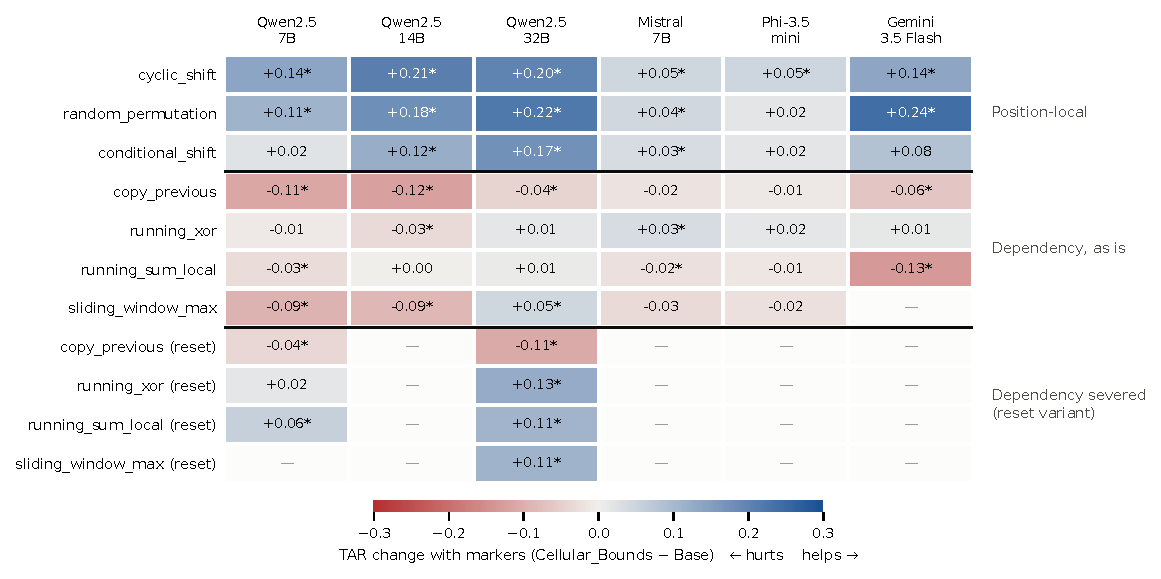
\includegraphics[width=\linewidth]{figures/fig1_split_heatmap.pdf}
\caption{Pooled change in token accuracy when markers are added (Bounds $-$ Base), every task and model. Pooled over $N \in \{4,\dots,64\}$, densities $k \in \{1,2,4,8,16\}$, and alphabet or modulus values. $^*$: $|z| \ge 2$. Blue: markers help; red: markers hurt; ---: not run. Top block: position-local tasks gain at every model. Middle block: the same markers produce no gain or a loss when they land on a dependency. Bottom block: the same dependency tasks rebuilt so the recurrence restarts at each marker (Section~\ref{sec:reset}). \pending{Qwen3.8-27B and Gemma-4-31B-it columns appear when their runs finish.}}
\label{fig:split}
\end{figure}

Figure~\ref{fig:split} shows the central result; per-model curves by length are in Appendix Figures~\ref{fig:tier1bymodel}--\ref{fig:harddep}. On position-local tasks (top block), all 18 cells are positive and 14 are significant. Averaged over the three tasks, the gain is +0.09 at Qwen2.5-7B, +0.17 at 14B, +0.20 at 32B, and +0.15 on Gemini. The gain is much smaller on Mistral-7B (+0.04) and Phi-3.5-mini (+0.03); for Mistral it also shrinks with length, reaching zero by $N = 64$ to $256$ in all three tasks (Appendix~\ref{app:models}).

On dependency tasks (middle block), the same markers give no comparable gain anywhere: none of the 23 cells exceeds +0.05, and 10 are significantly negative. Averaged over tasks, the effect is $-0.06$ at Qwen2.5-7B, 14B, and Gemini, and between $-0.01$ and $+0.01$ at Qwen2.5-32B, Mistral, and Phi. \task{copy\_previous}, which needs no computation, is hurt at every model, significantly at four of six, including where base accuracy is far above chance (Qwen2.5-14B: Base TAR 0.75 to 0.94).

The sign of the dependency effect varies with scale, but the gap between tiers does not. At Qwen2.5-32B, markers do not hurt three of four dependency tasks (\task{sliding\_window\_max} even gains +0.05), yet those tasks gain 0.15 to 0.19 less than the position-local average at the same model. We therefore frame the result as cancellation rather than harm: cutting a dependency offsets most of the benefit markers would otherwise bring (Section~\ref{sec:reset} measures this directly). Whether the net effect is positive or negative then depends on how large that benefit is for a given model.

\paragraph{External tasks.} The split holds on tasks we did not design (Appendix Tables~\ref{tab:external} and~\ref{tab:gemini}, Figures~\ref{fig:external} and~\ref{fig:geminifig}). On ProcBench's per-character substitution task \citep{fujisawa2024procbench}, markers help at both scales tested ($+0.054$, $z = 2.4$ at 7B; $+0.157$, $z = 5.9$ at 32B). On string copying \citep{jelassi2024repeat}, where base accuracy is already above 0.97, the effect is null, as expected with nothing to scaffold. On CLRS-Text's running-minimum algorithm \citep{markeeva2024clrstext}, a full-prefix dependency, markers hurt substantially wherever the model can do the task: $-0.25$ ($z = 5.1$) at Qwen2.5-32B and $-0.34$ ($z = 7.3$) on Gemini. Our one naturalistic position-local task is an exception: tagging each letter as vowel or consonant uses knowledge from pretraining rather than an in-context rule, and markers do not help it (7B: $-0.083$, $z = 2.3$; 32B: $+0.012$, $z = 0.5$).

% =====================================================================
\section{Severing the dependency restores the benefit}
\label{sec:reset}

If markers hurt dependency tasks because they sit between a position and the input it needs, removing that need should remove the cost. We rebuild each dependency task as a \emph{reset} variant: the position right after each marker is treated like the first position of the sequence, so the recurrence restarts at every marker and nothing before a marker is needed after it. The prompt states the new rule and gives a worked example (Appendix~\ref{app:prompts}), so the model attempts the reset task rather than being graded against answers it was not asked to produce. Lengths and densities match the originals.

\begin{figure}[t]
\centering
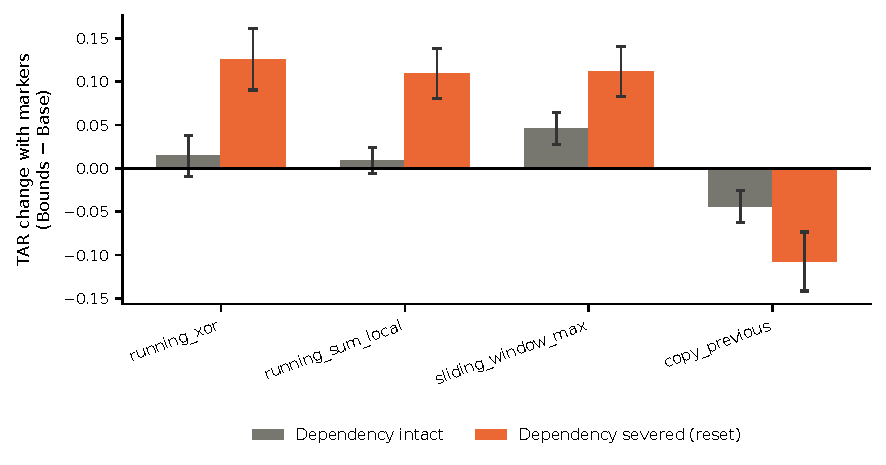
\includegraphics[width=0.75\linewidth]{figures/fig3_causal_only.pdf}
\caption{Severing the dependency restores the benefit (Qwen2.5-32B). Gray: markers inserted, dependency intact. Orange: the same task with the recurrence restarting at each marker. Three of four tasks move from near zero to $+0.11$ to $+0.13$. \task{copy\_previous} moves the other way because its reset rule alternates between two rules (see text).}
\label{fig:reset}
\end{figure}

\begin{table}[t]
\centering
\small
\caption{Reset ablation: TAR Base $\rightarrow$ Bounds, $\Delta$, and $|z|$, pooled as in Figure~\ref{fig:split}. Qwen2.5-7B: 40 trials per cell for originals, 80 for resets (two batches); Qwen2.5-32B: 20 to 40 per cell, single batch.}
\label{tab:reset}
\begin{tabular}{llcccc}
\toprule
& & \multicolumn{2}{c}{Original (dependency intact)} & \multicolumn{2}{c}{Reset (dependency severed)} \\
\cmidrule(lr){3-4}\cmidrule(lr){5-6}
Task & Model & Base$\rightarrow$Bounds & $\Delta$ ($|z|$) & Base$\rightarrow$Bounds & $\Delta$ ($|z|$) \\
\midrule
\multirow{2}{*}{\task{running\_xor}} & 7B & 0.410$\rightarrow$0.401 & $-$0.009 (0.7) & 0.465$\rightarrow$0.480 & +0.015 (1.5) \\
 & 32B & 0.781$\rightarrow$0.796 & +0.015 (1.2) & 0.749$\rightarrow$0.875 & +0.126 (6.9) \\
\multirow{2}{*}{\task{running\_sum\_local}} & 7B & 0.309$\rightarrow$0.279 & $-$0.030 (3.8) & 0.290$\rightarrow$0.347 & +0.057 (9.4) \\
 & 32B & 0.593$\rightarrow$0.602 & +0.009 (1.1) & 0.549$\rightarrow$0.659 & +0.110 (7.4) \\
\task{sliding\_window\_max} & 32B & 0.685$\rightarrow$0.731 & +0.046 (4.9) & 0.703$\rightarrow$0.814 & +0.112 (7.6) \\
\multirow{2}{*}{\task{copy\_previous}} & 7B & 0.529$\rightarrow$0.417 & $-$0.112 (7.4) & 0.587$\rightarrow$0.551 & $-$0.036 (3.3) \\
 & 32B & 0.858$\rightarrow$0.814 & $-$0.044 (4.6) & 0.897$\rightarrow$0.789 & $-$0.107 (6.2) \\
\bottomrule
\end{tabular}
\end{table}

Figure~\ref{fig:reset} and Table~\ref{tab:reset} show the result. At Qwen2.5-32B, \task{running\_xor}, \task{running\_sum\_local}, and \task{sliding\_window\_max} move from $+0.01$ to $+0.05$ with the dependency intact to $+0.11$ to $+0.13$ once it is severed, 56\% to 64\% of the position-local gain at the same model. Cutting the dependency had offset 59\% to 92\% of that restored gain. At 7B, \task{running\_sum\_local} reverses from a significant loss ($-0.030$) to a significant gain ($+0.057$), and \task{copy\_previous}'s loss shrinks by two-thirds. Six of seven task--model pairs move toward benefit.

\task{copy\_previous} at 32B is the exception, and the reset design explains it. Its reset rule alternates between ``copy the previous digit'' and ``copy this digit'' right after each marker, adding a rule switch at every marker. Errors in the reset condition concentrate on those switch positions. Because base accuracy is already high (0.86 to 0.90), there is little to gain and much to lose from that added complexity. The other three reset variants add no rule switch: restarting a sum, XOR, or window at a marker uses the same rule as the sequence start.

% =====================================================================
\section{Mechanism: markers are attention sinks held by positional heads}
\label{sec:mechanism}

We analyze Qwen2.5-32B on \task{cyclic\_shift}, using the real letter tokenization of the prompts.

\begin{figure}[t]
\centering
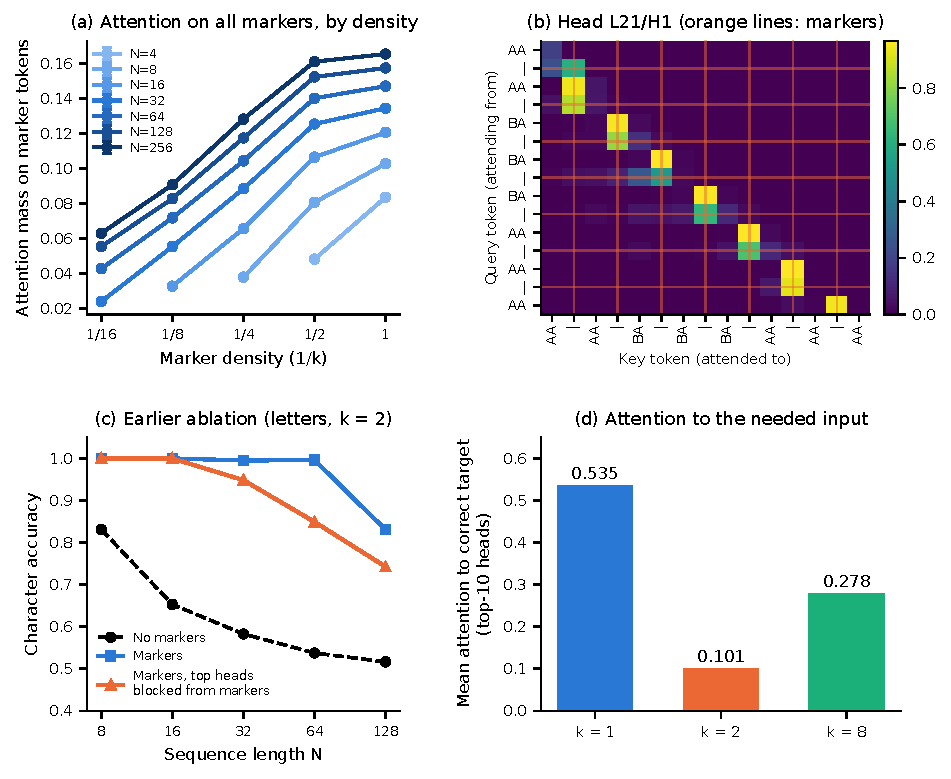
\includegraphics[width=\linewidth]{figures/fig2_mechanism_merged.pdf}
\caption{Mechanism (Qwen2.5-32B). (a) Attention mass on marker tokens rises with density at every length (\task{cyclic\_shift}, $A=2$). (b) The most marker-attending head (layer 21, head 1) attends from each position to an adjacent marker. (c) Masking the ten most marker-attending heads' attention to markers removes a growing share of the benefit as $N$ grows (0\% at $N \le 16$, 11\% at 32, 32\% at 64, 28\% at 128). (d) \task{copy\_previous} at $N=32$: mean attention from each output position to the input token it needs (top-10 heads) is 0.535 at $k=1$, collapses to 0.101 at the misaligned density $k=2$, and recovers to 0.278 at $k=8$, matching accuracy (Base 0.83; $k=1$: 0.88; $k=2$: 0.65; $k=8$: 0.84).}
\label{fig:mechanism}
\end{figure}

\paragraph{Markers attract attention in proportion to density.} The share of attention that lands on marker tokens rises monotonically with marker density at every length, roughly tripling from the sparsest to the densest setting (Figure~\ref{fig:mechanism}a). Individual heads attend sharply from each position to an adjacent marker (Figure~\ref{fig:mechanism}b; three such heads in Appendix Figure~\ref{fig:heads32b}), and attention entropy is higher with markers at nearly every layer (Appendix Figure~\ref{fig:attnmech}). The same pattern appears with a digit alphabet that tokenizes one character per token (Appendix Figure~\ref{fig:digits}), so it is not an artifact of letters merging into multi-character tokens.

\paragraph{The marker-attending heads are positional, not induction heads.} For the ten heads with the most attention to markers, we compute each head's percentile within the model on a standard induction-head test and on a positional (previous-token) test (Appendix Table~\ref{tab:heads}). Their mean induction percentile is 31 (none above 65), while their mean positional percentile is 95 (none below 83). Markers at fixed spacing are the kind of signal a positional head locks onto.

\paragraph{Blocking those heads from the markers removes the benefit.} At each length, we mask the attention from all positions to marker tokens in the ten most marker-attending heads, re-identified per length. At Qwen2.5-32B this removes 0\%, 0\%, 11\%, 32\%, and 28\% of the marker benefit at $N = 8, 16, 32, 64, 128$; at Qwen2.5-7B it removes 2\%, 35\%, 33\%, 63\%, and 74\% (Appendix Figure~\ref{fig:ablation7b32b}). The mechanism becomes load-bearing earlier and more completely in the smaller model; the larger model loses less, consistent with more redundant pathways. Two controls at 7B rule out a generic ablation cost. At $N = 16$ to $64$, masking ten random heads changes TAR by at most 0.006, and masking the same ten heads at random non-marker positions changes it by at most 0.023, against losses of 0.12 to 0.16 from the real ablation.

\paragraph{The same machinery explains the harm.} On \task{copy\_previous} at $N=32$, a density of one marker per character ($k=1$) keeps the marker pattern aligned with the one-step lookback, and attention from each output position to the input it needs is high (0.535, Figure~\ref{fig:mechanism}d). At $k=2$, every other lookback crosses a marker; attention to the needed token falls to 0.101 and accuracy drops from 0.88 to 0.65, below the no-marker baseline of 0.83. At $k=8$, fewer lookbacks cross a marker and both recover. The heads that make markers useful pull attention away from the input the dependency needs.

\paragraph{Errors recover after markers.} If markers act as reset points, a wrong output should be followed by a correct one more often when the next position comes right after a marker. On \task{cyclic\_shift} at Qwen2.5-32B, the next position is correct 89\% of the time after a marker versus 50\% otherwise at $N=16$, with the gap closing by $N = 128$ (Appendix Figure~\ref{fig:errorcontainment}). On a full-prefix sum task, where restarting locally is never valid, there is no consistent advantage.

% =====================================================================
\section{Practical considerations}
\label{sec:practical}

\paragraph{Density should fall as sequences grow.} The density that maximizes accuracy shifts toward sparser markers with length (Figure~\ref{fig:density}). On \task{cyclic\_shift} and \task{copy\_previous} at Qwen2.5-32B, a marker after every character is best through $N = 32$. At $N = 64$ and above, \task{cyclic\_shift} is best with a marker every second character, while \task{copy\_previous} keeps thinning to one marker per 8 characters at $N = 64$ and per 16 at $N = 128$. \task{sliding\_window\_max} has no single clean transition. We present this shift descriptively. A quadratic fit in density beats a linear one on held-out densities in only 42\% to 50\% of position-local curves and in none of 28 dependency-task curves (Appendix Table~\ref{tab:cv}); dependency tasks often have a worst density in the middle rather than a best one.

\begin{figure}[t]
\centering
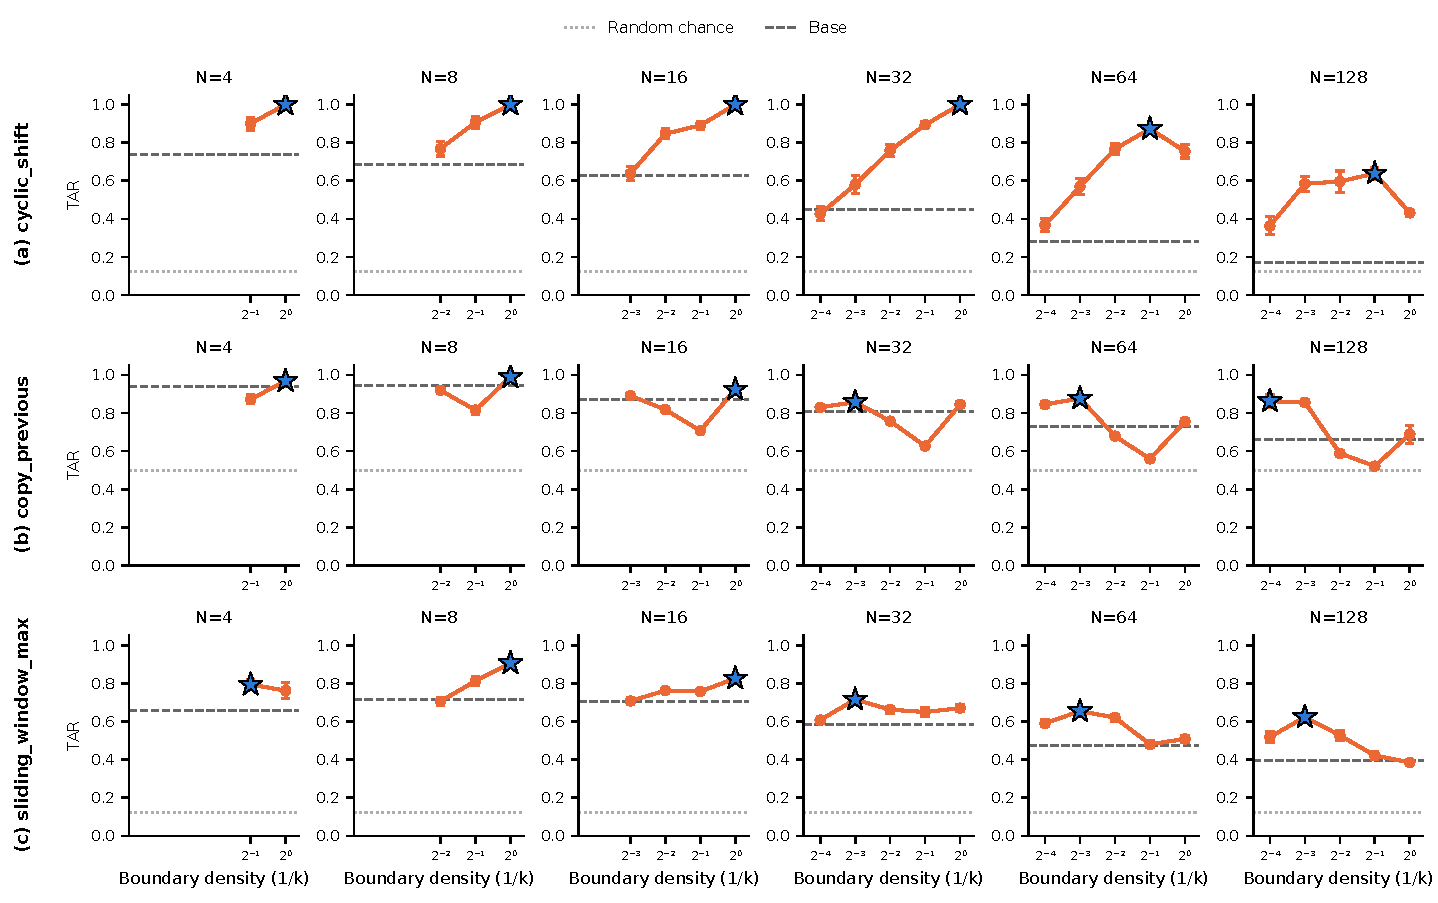
\includegraphics[width=\linewidth]{figures/fig2_vertex_migration.pdf}
\caption{Accuracy by marker density at each length (Qwen2.5-32B; $A = 8$ where applicable). Dashed: no-marker baseline; dotted: chance; star: best density. Dense markers win at short lengths, sparser markers at long lengths.}
\label{fig:density}
\end{figure}

\paragraph{Cost.} Generation speed is constant across conditions (14 to 15 tokens/s at Qwen2.5-32B), so wall-clock time tracks token count (Appendix Table~\ref{tab:wallclock}). The densest markers ($k=1$) take 3.4 times as long as no markers at $N=8$, falling to 1.3 times at $N=128$. Sparse markers ($k=8$) are faster than no markers at every length, at 0.66 times at $N=64$ and 0.44 times at $N=128$. True divide-and-conquer, with one call per segment (Appendix Figure~\ref{fig:dnc}), holds accuracy nearly flat (TAR 0.93 to 0.92 from $N=8$ to 128), but costs about three times the wall-clock of the marker condition at $N=64$ to 128. Markers recover much of that accuracy (0.87 to 0.75, against a no-marker baseline of 0.86 to 0.51) at close to the baseline's cost.

\paragraph{What about the marker matters.} Ablations on \task{cyclic\_shift} ($A = 2$, $k = 4$; Appendix Tables~\ref{tab:markerid}--\ref{tab:prompts}):
\begin{itemize}
\item \emph{Identity:} swapping \texttt{|} for \texttt{;} or \texttt{\#} changes little at Qwen2.5-32B.
\item \emph{Reserved tokens:} a reserved special token used as the marker performs far below the no-marker baseline at every length and both scales.
\item \emph{Frequency over token count:} a frequent single-token marker beats a less frequent multi-token marker that spends the same total number of tokens.
\item \emph{Regularity:} at 7B, jittered or random placement falls below the baseline at most lengths; at 32B both stay above it at every length.
\item \emph{Prompt wording:} the benefit holds under formal and casual phrasings of the instructions, but a terse cipher-style phrasing reverses it at 32B in four of five lengths.
\end{itemize}

\paragraph{A format tax.} Markers slightly reduce the fraction of outputs that are well formed (correct alphabet and full length) in six of seven tasks at Qwen2.5-32B, even where accuracy rises (Appendix Table~\ref{tab:wfr}). \task{random\_permutation} is the exception, improving on both measures. This cost is separate from the accuracy effect and should be checked when deploying markers.

% =====================================================================
\section{Limitations}
\label{sec:limitations}

\begin{itemize}
\item \textbf{Models.} \pending{The open models are 2024-era and instruction-tuned; Qwen3.8-27B and Gemma-4-31B-it runs are in progress.} We do not test base (non-instruct) models.
\item \textbf{Sample size.} The Qwen2.5-32B reset variants are single-batch (20 trials per cell). Gemini uses 3 trials per cell.
\item \textbf{Naturalistic tasks.} The one naturalistic position-local task (vowel tagging) shows no benefit. The position-local benefit is established for in-context rules, not yet for applying pretrained knowledge position by position.
\item \textbf{Reset design.} \task{copy\_previous}'s reset rule adds a rule switch, so it does not cleanly test severing that dependency.
\item \textbf{Dose--response shape.} The shift of the best density with length is descriptive; parametric fits do not generalize to held-out densities for dependency tasks.
\item \textbf{Prompt and marker sensitivity.} One prompt phrasing reverses the effect at 32B, and reserved special tokens do not work as markers.
\item \textbf{Mechanism scope.} Attention analyses are on Qwen2.5-7B and 32B only, and attention is tokenizer-dependent. Three of every four Qwen3.8-27B layers have no softmax attention, so the attention-sink account can apply only to its remaining 16 layers.
\end{itemize}

% =====================================================================
\section{Conclusion}
\label{sec:conclusion}

Inserting a content-free marker into the input every few characters is free in calls and nearly free in tokens. It reliably helps when each output depends only on its own position, because the markers become attention sinks that positional heads use to keep their place. The same machinery cancels the benefit when a marker sits between a position and the input it needs, and restarting the dependency at each marker brings the benefit back. Two simple rules follow for practitioners: use markers where computation is position-local, and place them, or restart the computation, so that they do not cut a dependency the task still needs.

\paragraph{Reproducibility.} \pending{Code, prompts, raw generations, and analysis scripts: anonymized repository link.} All inputs are generated from deterministic seeds, and every prompt can be regenerated from (task, length, density, alphabet, trial).

\bibliography{refs}
\bibliographystyle{tmlr}

% =====================================================================
\appendix

\section{Prompts}
\label{app:prompts}

\paragraph{\task{cyclic\_shift} ($N = 8$, $A = 4$, $k = 4$).}
\begin{small}
\begin{verbatim}
You are a deterministic sequence transformer.
Task: Cyclic character shift.
Alphabet: A, B, C, D
Rule: Replace every character with the next one in the alphabet.
Mapping: D -> A, and A -> B.
Constraint: The input contains vertical bars (|). These are structural
boundaries. DO NOT shift them. Copy them exactly to the output.
No spaces, no explanations.

Input: CABA|CCDA
Output:                 (expected: DBCB|DDAB)
\end{verbatim}
\end{small}

\paragraph{\task{running\_xor}, original and reset ($N = 8$, $k = 4$).} Both prompts state the rule $y_i = x_i \oplus x_{i-1}$ with the first digit copied. The reset prompt adds: \emph{``Immediately after each boundary, treat that position exactly like the first digit of the whole input---copy it as-is (nothing before a boundary counts as `previous'), then resume the XOR rule from there until the next boundary,''} with the worked example \texttt{1011|0010} $\rightarrow$ \texttt{1110|0011}. For input \texttt{1101|1111}, the original expects \texttt{1011|0000}, while the reset variant expects \texttt{1011|1000}: only the digit after the marker differs.

\paragraph{\task{sliding\_window\_max} ($N = 8$, $k = 4$).} The prompt states the rule with a worked example and adds: \emph{``DO NOT include them [the bars] in the window or count them as digits.''} For input \texttt{5170|1247} the expected output is \texttt{5577|7247}.

\section{Trials per cell}
\label{app:trials}

Table~\ref{tab:trials} gives trials per cell (one cell = task, model, length, density, and alphabet or modulus value) for the data pooled in Figure~\ref{fig:split}. Gemini uses 3. \pending{Add Qwen3.8-27B and Gemma-4-31B-it columns after their runs finish.}

\begin{table}[h]
\centering
\small
\caption{Trials per cell, $N \le 64$.}
\label{tab:trials}
\begin{tabular}{lccccc}
\toprule
Task & Qwen2.5-7B & Qwen2.5-14B & Qwen2.5-32B & Mistral-7B & Phi-3.5-mini \\
\midrule
\task{cyclic\_shift} & 20 & 20 & 20 & 40 & 20 \\
\task{random\_permutation} & 40 & 40 & 40 & 40 & 20 \\
\task{conditional\_shift} & 40 & 20 & 40 & 40 & 20 \\
\task{copy\_previous} & 40 & 40 & 80 & 40 & 40 \\
\task{running\_xor} & 40 & 40 & 40 & 40 & 20 \\
\task{running\_sum\_local} & 40 & 40 & 80 & 40 & 20 \\
\task{sliding\_window\_max} & 20 & 20 & 40 & 20 & 20 \\
Reset variants & 80 & -- & 20 & -- & -- \\
\bottomrule
\end{tabular}
\end{table}

\section{Per-model results}
\label{app:models}

\begin{figure}[h]
\centering
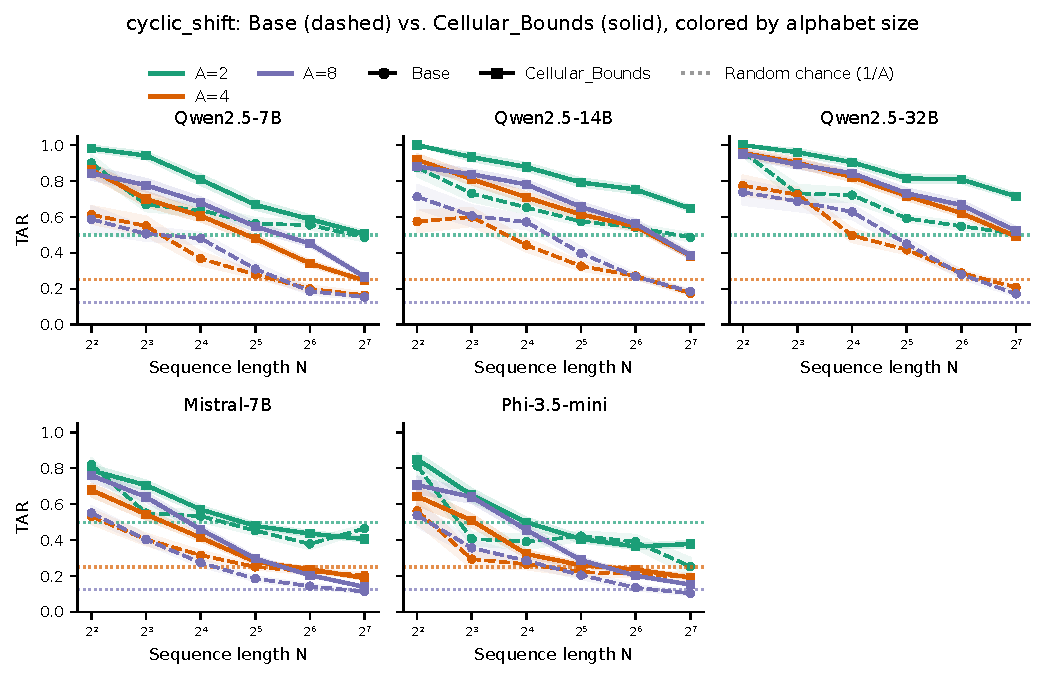
\includegraphics[width=\linewidth]{figures/tier1_cyclic_shift.pdf}
\caption{\task{cyclic\_shift} by model and length. Dashed: Base; solid: Bounds (pooled over densities); colors: alphabet size; dotted: chance.}
\label{fig:tier1bymodel}
\end{figure}

\begin{figure}[h]
\centering
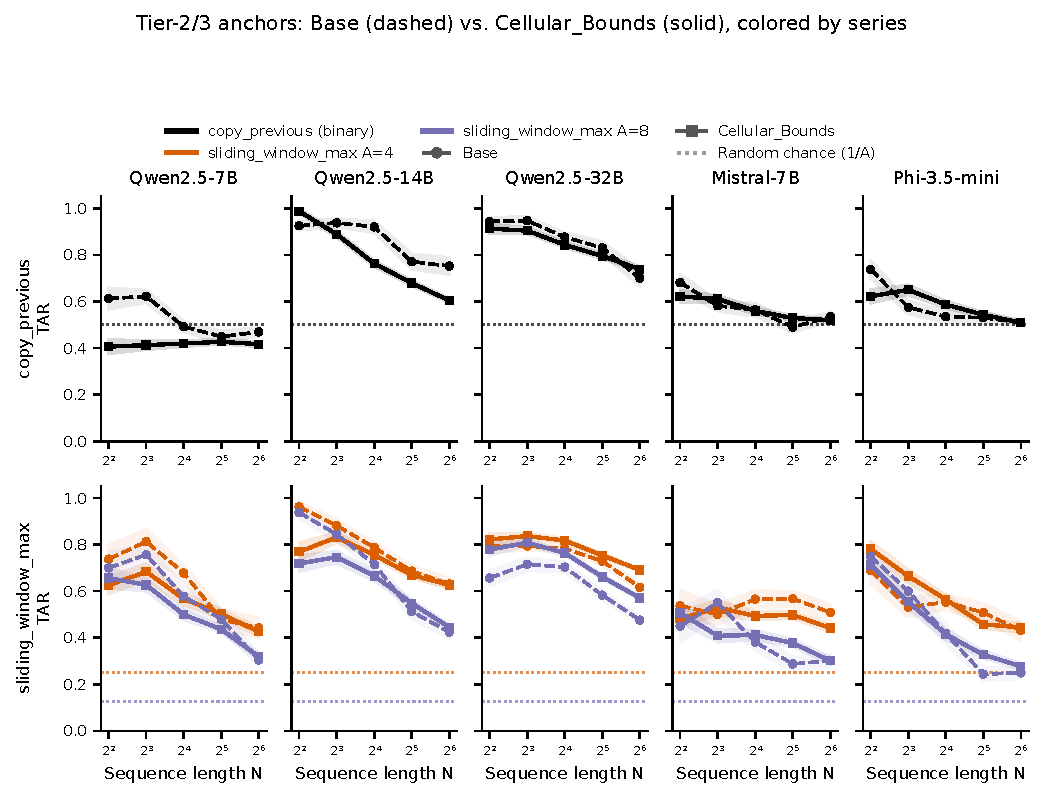
\includegraphics[width=\linewidth]{figures/anchors_grid.pdf}
\caption{\task{copy\_previous} and \task{sliding\_window\_max} by model. \task{copy\_previous} is hurt at most models; \task{sliding\_window\_max} is hurt at Qwen2.5-7B ($z = 4.6$), 14B ($z = 5.4$), Mistral, and Phi, and helped at Qwen2.5-32B ($z = 4.9$ with both seed batches; the curves shown are the first batch).}
\label{fig:anchors}
\end{figure}

\begin{figure}[h]
\centering
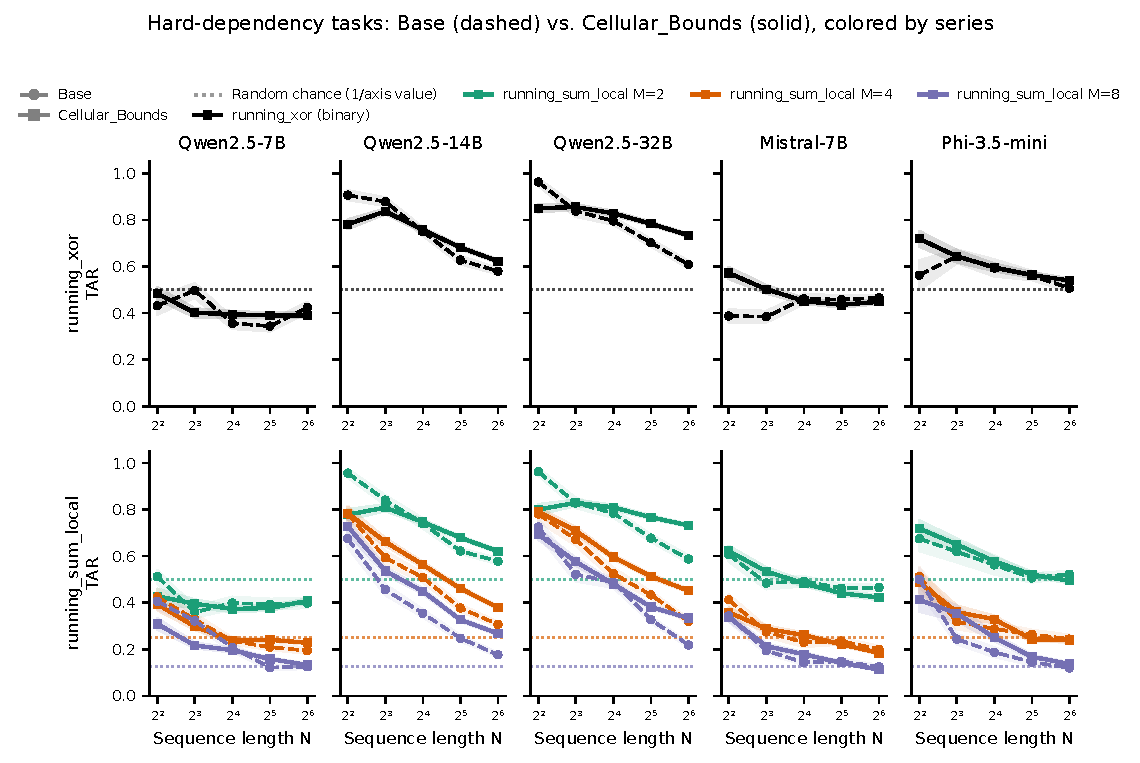
\includegraphics[width=\linewidth]{figures/hard_dependency_grid.pdf}
\caption{\task{running\_xor} and \task{running\_sum\_local} by model.}
\label{fig:harddep}
\end{figure}

\paragraph{Mistral-7B.} In all three position-local tasks, the benefit is largest at short lengths and decays to zero at the longest length tested (\task{cyclic\_shift}, $N=256$: $-0.003$, $z = 0.2$; \task{random\_permutation}, $N = 64$: $-0.012$, $z = 0.7$; \task{conditional\_shift}, $N=64$: $-0.011$, $z = 0.7$). In Qwen models the benefit holds or grows with length.

\paragraph{Repetition collapse.} On \task{running\_xor}, Qwen2.5-7B repeats a single wrong digit in about 38\% of trials, more often under dense markers. This failure falls to 0.9\% at 14B and 0.1\% for Mistral-7B, so it is specific to Qwen2.5-7B.

\section{External tasks}
\label{app:external}

\begin{table}[h]
\centering
\small
\caption{External position-local tasks, pooled across length and density. Best-$k$: TAR at the single best density (optimistic). $\Delta$: mean over all densities minus Base. $z$ as in Section~\ref{sec:setup}.}
\label{tab:external}
\begin{tabular}{lcccccc}
\toprule
& \multicolumn{3}{c}{Qwen2.5-7B} & \multicolumn{3}{c}{Qwen2.5-32B} \\
\cmidrule(lr){2-4}\cmidrule(lr){5-7}
Task & Base & Best-$k$ & $\Delta$ ($z$) & Base & Best-$k$ & $\Delta$ ($z$) \\
\midrule
Vowel/consonant tagging & 0.438 & 0.435 & $-$0.083 (2.3) & 0.615 & 0.657 & +0.012 (0.5) \\
ProcBench-Substitute & 0.196 & 0.422 & +0.054 (2.4) & 0.352 & 0.746 & +0.157 (5.9) \\
String copying & 0.972 & 0.983 & $-$0.006 (0.8) & 0.992 & 1.000 & $-$0.005 (1.6) \\
\bottomrule
\end{tabular}
\end{table}

\begin{table}[h]
\centering
\small
\caption{Closed-model check and CLRS-Text. Gemini 3.5 Flash with 3 trials per cell, pooled over all tested lengths (including $N$ up to 256 for \task{cyclic\_shift}). CLRS-Text tasks use token-level markers and scoring.}
\label{tab:gemini}
\begin{tabular}{llccc}
\toprule
Task & Model & Base TAR & Bounds TAR & $\Delta$ ($z$) \\
\midrule
\task{cyclic\_shift} & Gemini & 0.659 & 0.852 & +0.192 (5.0) \\
\task{random\_permutation} & Gemini & 0.606 & 0.846 & +0.240 (5.5) \\
\task{conditional\_shift} & Gemini & 0.544 & 0.628 & +0.084 (1.2) \\
\task{running\_xor} & Gemini & 0.900 & 0.913 & +0.013 (0.2) \\
\task{running\_sum\_local} & Gemini & 0.936 & 0.803 & $-$0.133 (5.6) \\
\task{copy\_previous} & Gemini & 0.988 & 0.924 & $-$0.064 (3.4) \\
\midrule
CLRS minimum & Qwen2.5-7B & 0.163 & 0.183 & +0.020 (1.1) \\
 & Qwen2.5-32B & 0.641 & 0.392 & $-$0.250 (5.1) \\
 & Gemini & 0.998 & 0.654 & $-$0.344 (7.3) \\
CLRS Kadane & Qwen2.5-7B & 0.076 & 0.068 & $-$0.008 (0.7) \\
 & Qwen2.5-32B & 0.214 & 0.122 & $-$0.092 (2.2) \\
 & Gemini & 0.391 & 0.354 & $-$0.037 (0.4) \\
\bottomrule
\end{tabular}
\end{table}

On Kadane's algorithm, base accuracy at both Qwen scales is statistically indistinguishable from chance under a shuffle test, so we do not interpret its effects. Minimum is well above chance at Qwen2.5-32B ($z = 4.1$ from shuffled chance).

\begin{figure}[h]
\centering
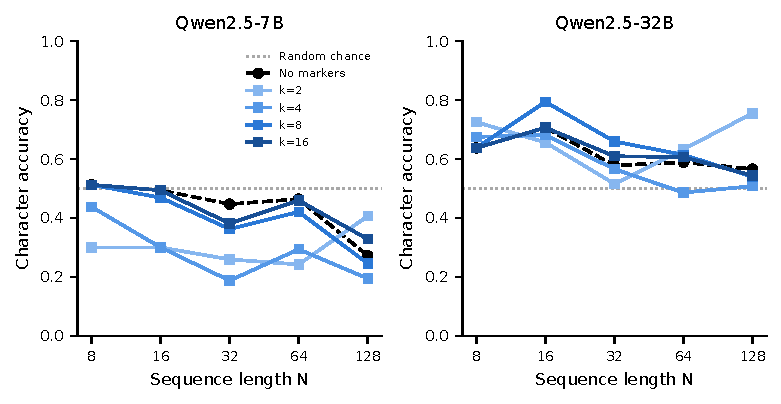
\includegraphics[width=0.32\linewidth]{figures/external_vowel_tagging.pdf}\hfill
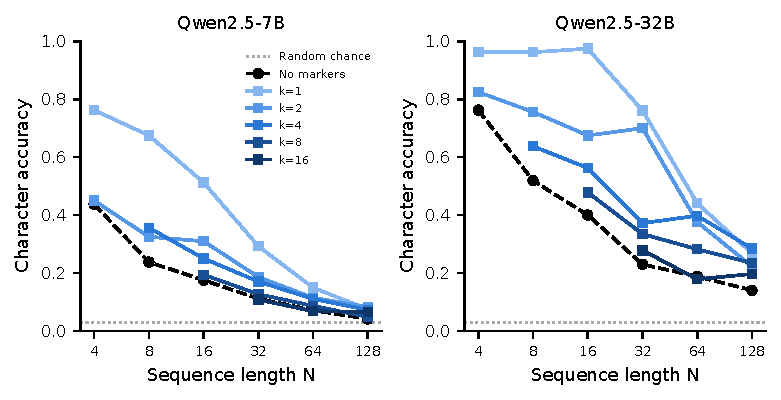
\includegraphics[width=0.32\linewidth]{figures/external_procbench.pdf}\hfill
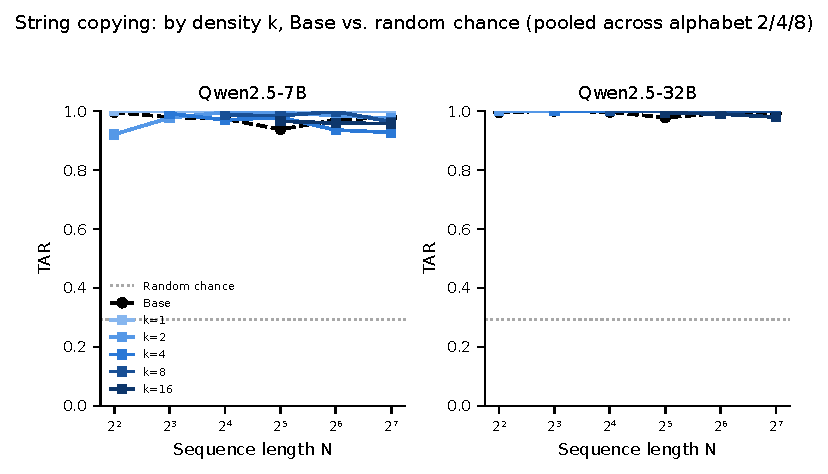
\includegraphics[width=0.32\linewidth]{figures/external_string_copy.pdf}
\caption{External position-local tasks by density. Left: vowel/consonant tagging. Middle: ProcBench-Substitute. Right: string copying.}
\label{fig:external}
\end{figure}

\begin{figure}[h]
\centering
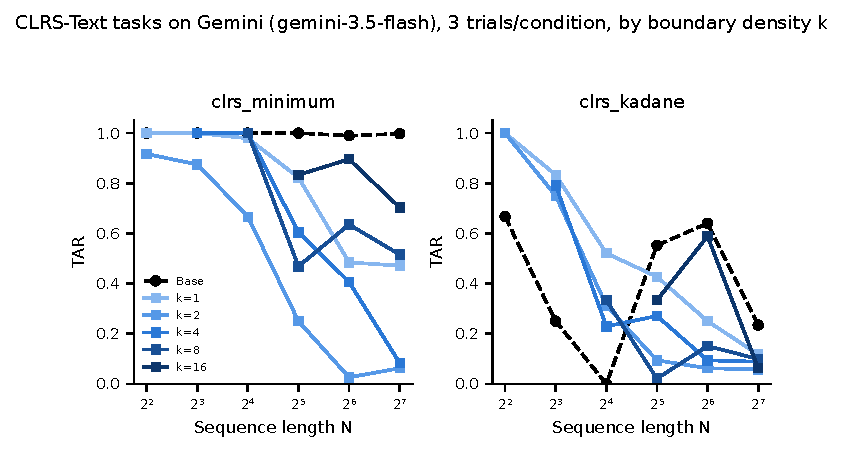
\includegraphics[width=\linewidth]{figures/external_benchmark_gemini.pdf}
\caption{Gemini 3.5 Flash by task and density, with CLRS-Text tasks across models.}
\label{fig:geminifig}
\end{figure}

\section{Mechanism details}
\label{app:mechanism}

\begin{figure}[h]
\centering
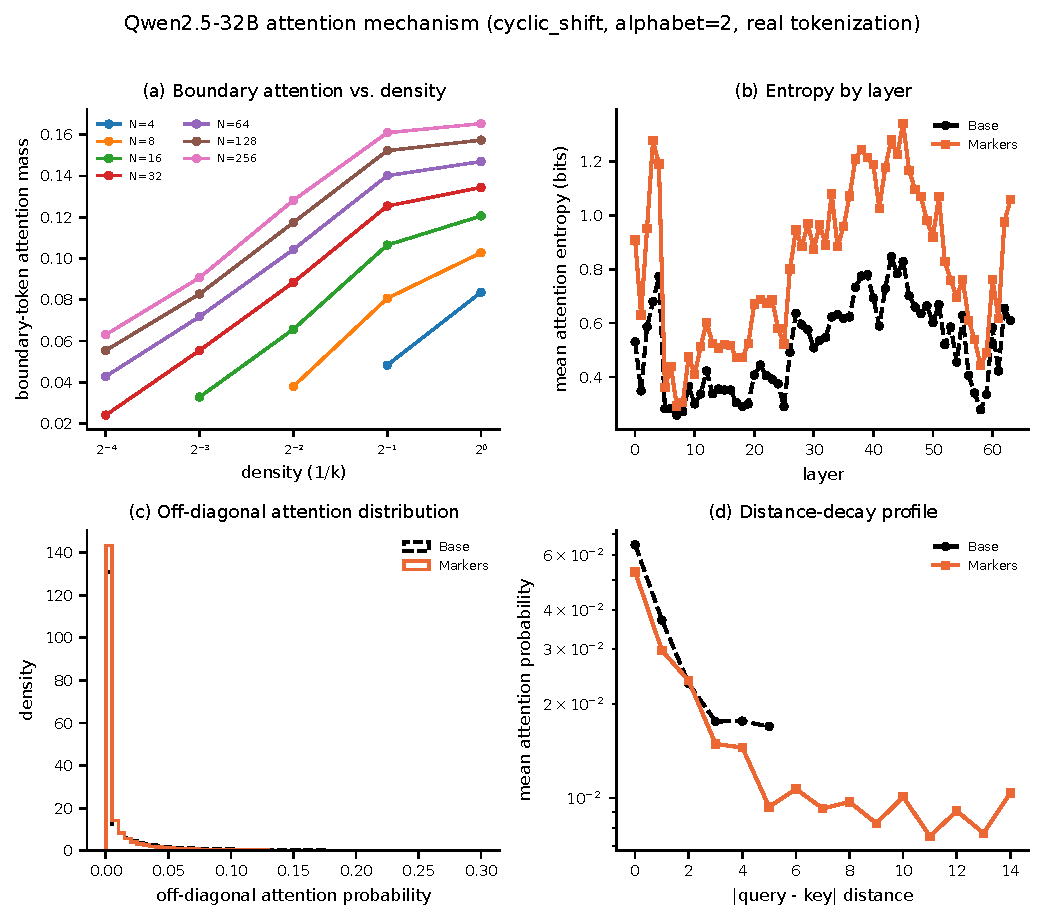
\includegraphics[width=\linewidth]{figures/attention_mechanism_32b.pdf}
\caption{Attention analysis, Qwen2.5-32B, \task{cyclic\_shift}: marker attention by density, attention entropy by layer (higher under markers at nearly every layer), off-diagonal attention, and distance decay.}
\label{fig:attnmech}
\end{figure}

\begin{figure}[h]
\centering
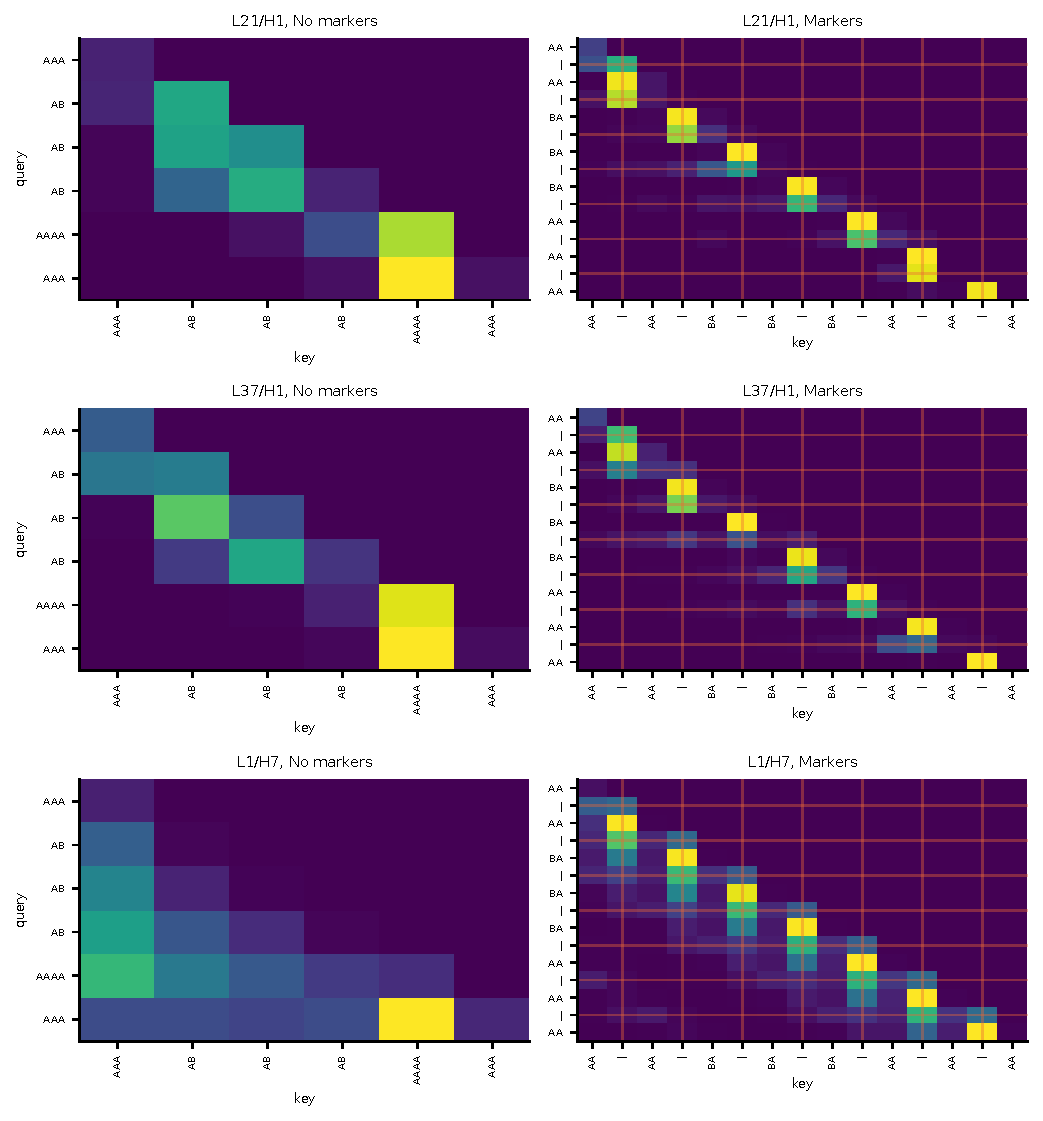
\includegraphics[width=\linewidth]{figures/head_heatmaps_32b.pdf}
\caption{The three most marker-attending heads at Qwen2.5-32B (L21/H1, L37/H1, L1/H7). Without markers, letters merge into multi-character tokens; markers restore per-character resolution.}
\label{fig:heads32b}
\end{figure}

\begin{figure}[h]
\centering
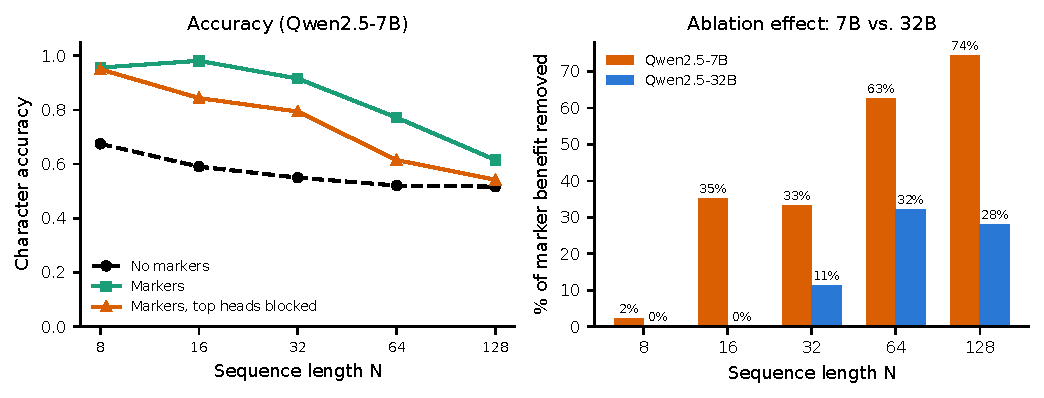
\includegraphics[width=\linewidth]{figures/causal_ablation.pdf}
\caption{Head ablation at Qwen2.5-7B and 32B: share of the marker benefit removed by masking the ten most marker-attending heads' attention to markers, re-identified at each length.}
\label{fig:ablation7b32b}
\end{figure}

\begin{figure}[h]
\centering
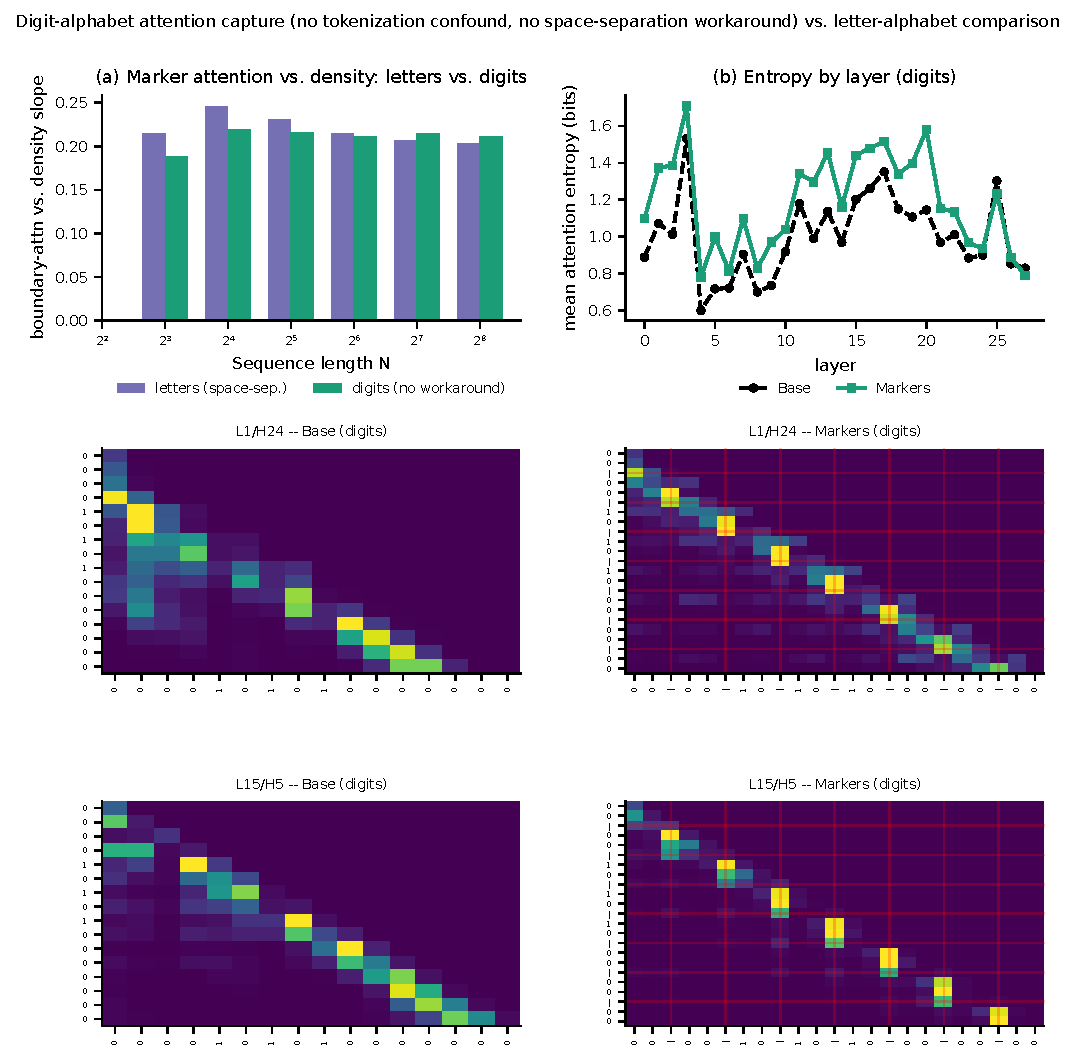
\includegraphics[width=\linewidth]{figures/attention_digits_comparison.pdf}
\caption{Tokenization check: marker-attention slopes with letters (space-separated, one token per letter) and digits (natively one token per character) are nearly identical.}
\label{fig:digits}
\end{figure}

\begin{figure}[h]
\centering
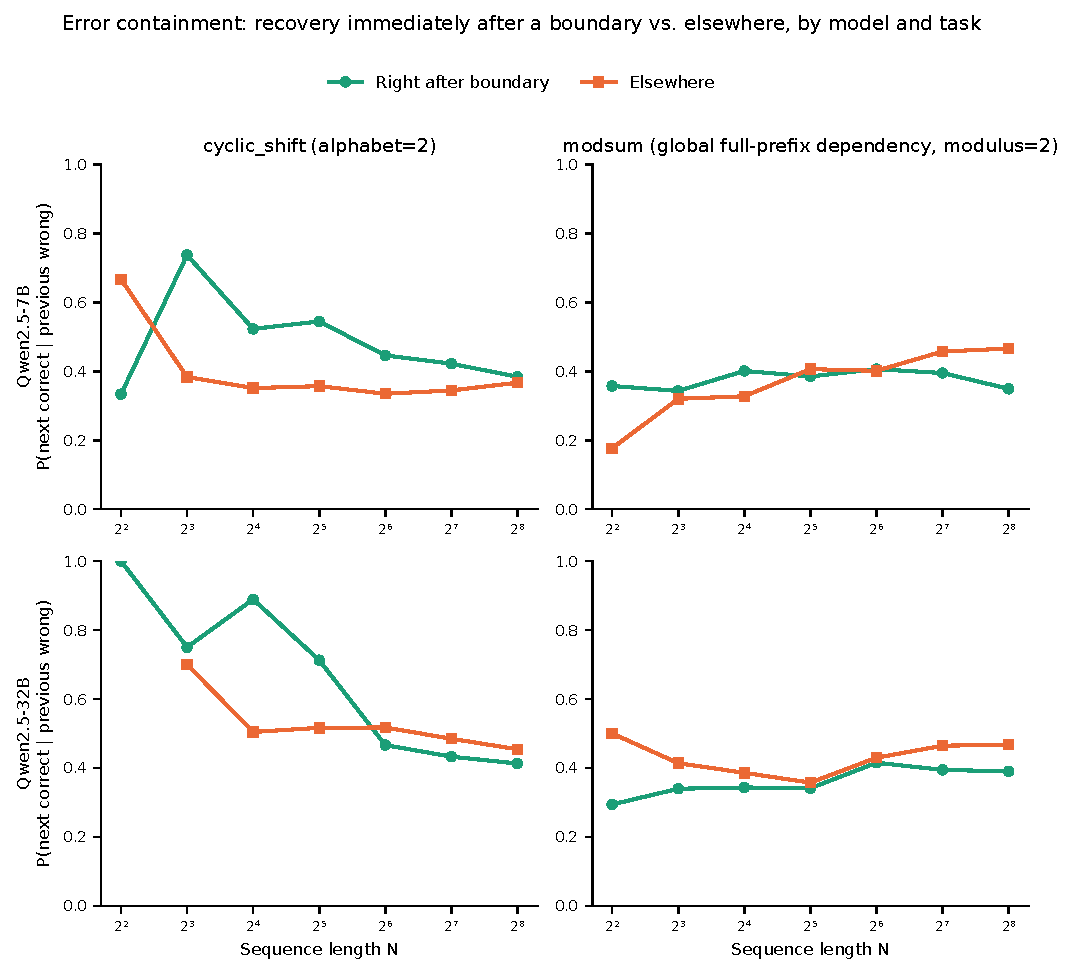
\includegraphics[width=\linewidth]{figures/error_containment_combined.pdf}
\caption{Error recovery: after a wrong output, the fraction of next positions that are correct, split by whether the next position follows a marker. Left: \task{cyclic\_shift}; right: a full-prefix modular sum. $A = M = 2$.}
\label{fig:errorcontainment}
\end{figure}

\begin{table}[h]
\centering
\small
\caption{The ten most marker-attending heads at Qwen2.5-32B, with percentiles within all heads on an induction test and a positional (previous-token) test.}
\label{tab:heads}
\begin{tabular}{cccc}
\toprule
Layer/Head & Marker attention & Induction pct. & Positional pct. \\
\midrule
21/1 & 0.099 & 38.3 & 98.3 \\
37/1 & 0.087 & 47.4 & 96.7 \\
1/7 & 0.086 & 17.1 & 97.7 \\
35/19 & 0.082 & 23.1 & 96.5 \\
35/3 & 0.080 & 14.7 & 97.2 \\
30/32 & 0.079 & 18.6 & 96.0 \\
32/37 & 0.075 & 14.3 & 98.8 \\
1/8 & 0.072 & 64.8 & 97.7 \\
32/7 & 0.071 & 60.4 & 90.2 \\
19/19 & 0.068 & 9.9 & 83.9 \\
\midrule
Mean & & 30.9 & 95.3 \\
\bottomrule
\end{tabular}
\end{table}

\section{Marker ablations}
\label{app:marker}

\begin{table}[h]
\centering
\small
\caption{Marker identity, reserved token, and token budget (\task{cyclic\_shift}, $A = 2$, periodic $k = 4$ unless noted). TAR. Budget-matched: \texttt{<|>} at $k = 12$ uses the same total tokens as \texttt{|} at $k = 4$.}
\label{tab:markerid}
\begin{tabular}{llcccccc}
\toprule
$N$ & Model & Base & \texttt{|} & \texttt{;} & \texttt{\#} & Reserved token & \texttt{<|>}, $k=12$ \\
\midrule
\multirow{2}{*}{8} & 7B & 0.675 & 0.717 & 0.792 & 0.792 & 0.469 & 0.675 \\
 & 32B & 0.831 & 0.892 & 0.942 & 0.908 & 0.525 & 0.806 \\
\multirow{2}{*}{16} & 7B & 0.591 & 0.825 & 0.750 & 0.667 & 0.216 & 0.591 \\
 & 32B & 0.653 & 0.896 & 0.846 & 0.912 & 0.284 & 0.759 \\
\multirow{2}{*}{32} & 7B & 0.550 & 0.679 & 0.769 & 0.585 & 0.092 & 0.539 \\
 & 32B & 0.583 & 0.848 & 0.781 & 0.744 & 0.186 & 0.688 \\
\multirow{2}{*}{64} & 7B & 0.521 & 0.616 & 0.650 & 0.591 & 0.049 & 0.453 \\
 & 32B & 0.537 & 0.759 & 0.658 & 0.693 & 0.160 & 0.710 \\
\multirow{2}{*}{128} & 7B & 0.517 & 0.545 & 0.507 & 0.496 & 0.046 & 0.452 \\
 & 32B & 0.516 & 0.694 & 0.744 & 0.561 & 0.219 & 0.642 \\
\bottomrule
\end{tabular}
\end{table}

\begin{table}[h]
\centering
\small
\caption{Placement regularity (\task{cyclic\_shift}, $A = 2$, marker count matched to $k = 4$). TAR.}
\label{tab:jitter}
\begin{tabular}{c ccccc ccccc}
\toprule
& \multicolumn{5}{c}{Qwen2.5-7B} & \multicolumn{5}{c}{Qwen2.5-32B} \\
\cmidrule(lr){2-6}\cmidrule(lr){7-11}
$N$ & Base & Periodic & $\pm 1$ & $\pm 2$ & Random & Base & Periodic & $\pm 1$ & $\pm 2$ & Random \\
\midrule
8 & 0.675 & 0.717 & 0.581 & 0.675 & 0.633 & 0.831 & 0.892 & 0.869 & 0.912 & 0.858 \\
16 & 0.591 & 0.825 & 0.572 & 0.566 & 0.583 & 0.653 & 0.896 & 0.863 & 0.787 & 0.733 \\
32 & 0.550 & 0.679 & 0.572 & 0.509 & 0.552 & 0.583 & 0.848 & 0.847 & 0.745 & 0.779 \\
64 & 0.521 & 0.616 & 0.502 & 0.491 & 0.491 & 0.537 & 0.759 & 0.731 & 0.732 & 0.682 \\
128 & 0.517 & 0.545 & 0.493 & 0.471 & 0.452 & 0.516 & 0.694 & 0.691 & 0.695 & 0.583 \\
\bottomrule
\end{tabular}
\end{table}

\begin{table}[h]
\centering
\small
\caption{Prompt wording (\task{cyclic\_shift}, $A = 2$, $k = 4$, 15 trials per cell). $\Delta$ = Bounds $-$ Base TAR.}
\label{tab:prompts}
\begin{tabular}{l ccccc ccccc}
\toprule
& \multicolumn{5}{c}{Qwen2.5-7B, $N =$} & \multicolumn{5}{c}{Qwen2.5-32B, $N =$} \\
\cmidrule(lr){2-6}\cmidrule(lr){7-11}
Wording & 8 & 16 & 32 & 64 & 128 & 8 & 16 & 32 & 64 & 128 \\
\midrule
Formal & +.09 & +.27 & +.10 & +.13 & +.07 & +.26 & +.17 & +.17 & +.20 & +.18 \\
Casual & $-$.04 & +.08 & +.12 & +.04 & +.10 & +.08 & +.25 & +.17 & +.21 & +.20 \\
Terse cipher & $-$.07 & +.08 & +.00 & +.00 & +.05 & $-$.12 & $-$.11 & +.01 & $-$.07 & $-$.05 \\
\bottomrule
\end{tabular}
\end{table}

\section{Dose--response robustness}
\label{app:dose}

\begin{table}[h]
\centering
\small
\caption{Does a quadratic in density describe accuracy curves? ``AIC'': share of curves where a quadratic beats linear and exponential fits in-sample. ``Held-out'': share where it also beats a linear fit on leave-one-density-out prediction.}
\label{tab:cv}
\begin{tabular}{llcccc}
\toprule
Task & Tier & Curves & Mean quadratic $R^2$ & AIC & Held-out \\
\midrule
\task{cyclic\_shift} & position-local & 15 & 0.876 & 93\% & 47\% \\
\task{random\_permutation} & position-local & 12 & 0.941 & 92\% & 42\% \\
\task{conditional\_shift} & position-local & 12 & 0.908 & 100\% & 50\% \\
\task{copy\_previous} & one-step & 4 & 0.608 & 50\% & 0\% \\
\task{running\_xor} & one-step & 4 & 0.449 & 25\% & 0\% \\
\task{running\_sum\_local} & one-step & 12 & 0.512 & 42\% & 0\% \\
\task{sliding\_window\_max} & windowed & 8 & 0.473 & 50\% & 0\% \\
\bottomrule
\end{tabular}
\end{table}

\section{Well-formedness and cost}
\label{app:wfr}

\begin{table}[h]
\centering
\small
\caption{Well-formedness at Qwen2.5-32B. VVR: share of outputs using only the task alphabet. CR: share at least as long as the answer. WFR: share satisfying both. Pooled across lengths and alphabets.}
\label{tab:wfr}
\begin{tabular}{llccccc}
\toprule
Task & Condition & Trials & TAR & VVR & CR & WFR \\
\midrule
\multirow{2}{*}{\task{cyclic\_shift}} & Base & 420 & 0.511 & 0.536 & 0.919 & 0.521 \\
 & Bounds & 1740 & 0.701 & 0.568 & 0.806 & 0.444 \\
\multirow{2}{*}{\task{random\_permutation}} & Base & 600 & 0.499 & 0.995 & 0.858 & 0.855 \\
 & Bounds & 2280 & 0.720 & 0.994 & 0.923 & 0.918 \\
\multirow{2}{*}{\task{conditional\_shift}} & Base & 300 & 0.514 & 0.917 & 0.937 & 0.863 \\
 & Bounds & 1140 & 0.671 & 0.834 & 0.908 & 0.752 \\
\multirow{2}{*}{\task{running\_xor}} & Base & 200 & 0.781 & 1.000 & 0.940 & 0.940 \\
 & Bounds & 760 & 0.796 & 1.000 & 0.930 & 0.930 \\
\multirow{2}{*}{\task{running\_sum\_local}} & Base & 600 & 0.590 & 0.830 & 0.900 & 0.765 \\
 & Bounds & 2280 & 0.601 & 0.699 & 0.946 & 0.675 \\
\multirow{2}{*}{\task{copy\_previous}} & Base & 200 & 0.859 & 1.000 & 0.955 & 0.955 \\
 & Bounds & 760 & 0.817 & 1.000 & 0.879 & 0.879 \\
\multirow{2}{*}{\task{sliding\_window\_max}} & Base & 200 & 0.684 & 1.000 & 0.995 & 0.995 \\
 & Bounds & 760 & 0.727 & 1.000 & 0.943 & 0.943 \\
\bottomrule
\end{tabular}
\end{table}

\begin{table}[h]
\centering
\small
\caption{Wall-clock seconds per call at Qwen2.5-32B. Throughput is 14 to 15 tokens/s in every condition.}
\label{tab:wallclock}
\begin{tabular}{lcccccc}
\toprule
Condition & $k$ & $N=8$ & 16 & 32 & 64 & 128 \\
\midrule
Base & -- & 0.330 & 0.570 & 1.270 & 3.763 & 11.380 \\
Bounds & 1 & 1.133 & 2.215 & 4.403 & 7.684 & 14.260 \\
Bounds & 2 & 0.544 & 1.076 & 2.142 & 4.213 & 9.000 \\
Bounds & 4 & 0.380 & 0.787 & 1.729 & 3.298 & 6.453 \\
Bounds & 8 & 0.312 & 0.613 & 1.288 & 2.479 & 4.976 \\
\bottomrule
\end{tabular}
\end{table}

\begin{figure}[h]
\centering
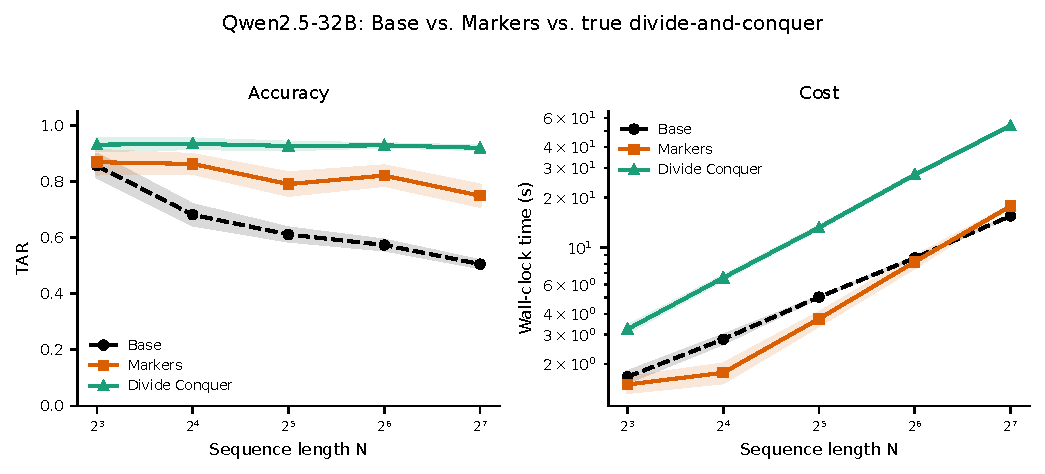
\includegraphics[width=0.8\linewidth]{figures/divide_and_conquer.pdf}
\caption{Markers versus true divide-and-conquer (one call per segment), Qwen2.5-32B: accuracy and wall-clock by length.}
\label{fig:dnc}
\end{figure}

\end{document}
